
\documentclass[13pt,a4paper]{report}
\usepackage[margin=0.6in]{geometry}
\usepackage{fancybox}
\usepackage[utf8]{inputenc}
\usepackage[vietnamese,main=english]{babel}
\usepackage{multicol}
\usepackage{tabularx}
\usepackage{lmodern}
\usepackage{minted}
\usepackage{indentfirst}
\usepackage{float}
\usepackage{enumitem}
\usepackage{afterpage}
\usepackage[super]{nth}
\usepackage{titlesec}
\usepackage{bigdelim}
\usepackage[titles]{tocloft}
\usepackage{makecell}
\usepackage{arydshln}
\usepackage{perpage} %the perpage package
\usepackage{graphicx}
\usepackage{caption}
\usepackage{gensymb}
\usepackage{tikz}
\usepackage{circuitikz}
\usepackage{pgfplots}
\usepackage{cancel}
\usepackage{xurl}
\usepackage[bottom]{footmisc}
\usepackage[font=footnotesize,labelfont={scriptsize}]{subfig}
\usepackage{wrapfig}
\usepackage{latexsym,amssymb,amsmath}
%\usepackage{algpseudocode}
\usepackage{tocvsec2}
\usepackage{fancyref}
\usepackage{bookmark}
\usepackage{hyperref}
\usepackage[nameinlink,noabbrev]{cleveref}

\newcolumntype{Y}{>{\centering\arraybackslash}X}

\PassOptionsToPackage{hyphens}{url}

\makeatletter
\pgfcircdeclarebipole{}{\ctikzvalof{bipoles/vsourceam/height}}{vsourceAM}{\ctikzvalof{bipoles/vsourceam/height}}{\ctikzvalof{bipoles/vsourceam/width}}{%
  \pgfsetlinewidth{\pgfkeysvalueof{/tikz/circuitikz/bipoles/thickness}\pgfstartlinewidth}
   \pgfpathellipse{\pgfpointorigin}{\pgfpoint{0}{\pgf@circ@res@up}}{\pgfpoint{\pgf@circ@res@left}{0}}
   \pgfusepath{draw}
   \pgfscope
       \pgftransformxshift{0.6*\ctikzvalof{bipoles/vsourceam/margin}\pgf@circ@res@left}
       \pgftext[rotate=-\pgf@circ@direction]{$+$}
       \pgfusepath{draw}
   \endpgfscope
   \pgfscope
       \pgftransformxshift{0.6*\ctikzvalof{bipoles/vsourceam/margin}\pgf@circ@res@right}
       \pgftext[rotate=-\pgf@circ@direction]{$-$}
       \pgfusepath{draw}
   \endpgfscope
}
\makeatother

\MakePerPage{footnote} %the perpage package command
\usetikzlibrary{shapes,positioning,arrows,calc}

\newcommand*\justify{%
  \fontdimen2\font=0.4em% interword space
  \fontdimen3\font=0.2em% interword stretch
  \fontdimen4\font=0.1em% interword shrink
  \fontdimen7\font=0.1em% extra space
  \hyphenchar\font=`\-% allowing hyphenation
}
\renewcommand\cftchapafterpnum{\vskip-2pt}
\renewcommand\cftsecafterpnum{\vskip-2pt}

\renewcommand{\theequation}{\arabic{equation}}

% FLOW CHART
\tikzstyle{startstop} = [rectangle, rounded corners, minimum width=3cm, minimum height=1cm,text centered, draw=black, fill=red!30]
\tikzstyle{io} = [trapezium, trapezium left angle=70, trapezium right angle=110, minimum width=3cm, minimum height=1cm, text centered, draw=black, fill=blue!30]
\tikzstyle{process} = [rectangle, minimum width=3cm, minimum height=1cm, text centered, draw=black, fill=orange!30, text width=4cm]
\tikzstyle{decision} = [diamond, aspect=2.5, minimum width=3cm, minimum height=1cm, text centered, draw=black, fill=green!30]
\tikzstyle{arrow} = [thick,->,>=stealth]

% CHAPTER FORMAT
\titleformat{\chapter}%[display]
{\bfseries\fontsize{25}{30}\selectfont\raggedright}% Format and size of title text
{\llap{%
    \rule[-6pt]{6cm}{1.18cm}\rule{6pt}{0pt}}% Black box to the left, lowered 6pt. The end rule is a horisontal space.
  \llap{% Number also to the left, on top of the black box.
    \fontsize{30}{44}\selectfont\color{white}\thechapter\rule{10pt}{0pt}}}{0pt}{}{}

\counterwithin{figure}{section}
\renewcommand{\thefigure}{\arabic{chapter}.\arabic{section}.\alph{figure}}

\renewcommand{\thetable}{\arabic{table}}

\renewcommand\labelitemi{$-$}
  
\titleformat{\section}
  {\LARGE\bfseries}{}{}{}
\renewcommand\thesection{\arabic{section}.}
\renewcommand\thesubsection{\arabic{subsection}}
\makeatletter
\renewcommand*\l@section{\@dottedtocline{1}{1.5cm}{2em}}
\renewcommand\section{\@startsection {section}{1}{-1em}%
  {-3.5ex \@plus -1ex \@minus -.2ex}%
  {2.3ex \@plus.2ex}%
  {\normalfont\Large\bfseries}}
\def\sectionmark#1{%
      \markright {\MakeUppercase{#1}}}
\makeatother

\titleformat{\subsection}
  {\normalfont\bfseries}{\thesubsection.}{0.5em}{}
\renewcommand\cftsubsecaftersnum{.} 
\renewcommand\thesubsection{\alph{subsection}}

\addto{\captionsenglish}{%
  \renewcommand{\bibname}{References}
}

%\addtocontents{toc}{\setcounter{tocdepth}{2}}
%\addtocontents{lof}{\vskip -1.6cm}
%\addtocontents{lot}{\vskip -1.6cm}

    
% TOC settings
\renewcommand\cftchapnumwidth{2.8em}
\renewcommand\cftsecnumwidth{3em}
\renewcommand\cftsecindent{3em}
\renewcommand\cftsubsecindent{5em}
\renewcommand\thechapter{\Roman{chapter}}
    
%\titleformat{\chapter}[display]{\normalfont\huge\bfseries}{}{0pt}{\Huge}
\newcommand{\hsp}{\hspace{20pt}}
%\titleformat{\chapter}[hang]{\Huge\bfseries}{\thechapter\hsp\textcolor{gray75}{|}\hsp}{0pt}{\Huge\bfseries}
\titleformat*{\subsubsection}{\large\bfseries}
%\titlespacing*{\chapter}{0pt}{0pt}{0pt}
    
\newcolumntype{P}[1]{>{\centering\arraybackslash}p{#1}}
\newcolumntype{C}{>{\centering\arraybackslash}p{4em}}
    
\setlist[itemize]{noitemsep, topsep=0pt}
%\AtBeginEnvironment{multicols}{\RaggedRight}

\titlespacing*{\chapter}{0pt}{0pt}{20pt}

\newcommand\Chapter[2]{\chapter
  [#1\text{: }\hfil\hbox{}\protect\linebreak{\itshape#2}]%
  {#1\\[-0.75ex]\Large#2}%
  \markboth{\MakeUppercase{\chaptername\ \thechapter.\ #1}}{}%
}


\def\doubleoverline#1{\overline{\overline{#1}}}

\captionsetup[subfloat]{labelformat=empty}

\begin{document}
%Trang bìa 1
\fontsize{13pt}{18pt}\selectfont
\begin{titlepage}
\thispagestyle{empty}
\thisfancypage{%đóng khung trang này
\setlength{\fboxsep}{0pt}% 8pt là độ dày của đường viền
\fbox}{} % phần nội dung sau là tương tự như đã làm
\

\begin{center}
\begin{large}
HO CHI MINH CITY UNIVERSITY OF TECHNOLOGY $-$ VNU HCMC
\end{large} \\
\begin{large}
OFFICE FOR INTERNATIONAL STUDY PROGRAM
\end{large} \\
\begin{large}
FACULTY OF ELECTRICAL AND ELECTRONIC ENGINEERING
\end{large} \\
\textbf{--------------------  *  --------------------}\\[4cm]

\includegraphics[scale=0.1]{logobk.png}\\[1cm]
{\fontsize{20pt}{1}\selectfont DIGITAL SYSTEMS (LAB)}\\
{\fontsize{20pt}{1}\selectfont EXPERIMENTAL REPORT (Lab 1)}\\[2.5cm]
\end{center}

\begin{otherlanguage}{vietnamese}
\begin{tabbing}
	\hspace{3.5cm}Lecturer  \ \ \ \ \=: \textbf{\parbox[t]{9cm}{Mr. Nguyễn Tuấn Hùng}}\\
	\hspace{3.5cm}Subject \>: \textbf{\parbox[t]{12cm}{Digital Systems}}\\
	\hspace{3.5cm}Class \>: \textbf{\parbox[t]{9cm}{TT06}}\\
	\hspace{3.5cm}Name \>: \textbf{\parbox[t]{9cm}{
		Lương Triển Thắng}}\\
	\hspace{3.5cm}Student ID \>: \textbf{\parbox[t]{9cm}{
		2051194}}\\[40pt]
\end{tabbing}
\end{otherlanguage}

\vspace{2.25cm}
\begin{center}
{\fontsize{13pt}{1}\selectfont Ho Chi Minh City, \nth{31} May, 2022}
\end{center}
\end{titlepage}

\tableofcontents

\setminted{fontsize=\normalsize}

\setcounter{chapter}{0}

\Chapter{Laboratory 1}{Get started with FPGA}

\section{Know how to program $n$-bit wide 2-to-1 multiplexer}

\ctikzset{logic ports=ieee}

\begin{figure}[H]
\centering
\begin{circuitikz}
\tikzset{mux21/.style={muxdemux, muxdemux def={NL=2, NB=0, NT=1, NR=1, Lh=6, Rh=3, w=1.5}}}

\draw
  (0,0) node[mux21] (mux21) {}
  
  (mux21.lpin 1) to [multiwire=4] ++(-1,0) node[anchor=east] {$x$}
  (mux21.lpin 2) to [multiwire=4] ++(-1,0) node[anchor=east] {$y$}
  (mux21.rpin 1) to [multiwire=4] ++(1,0) node[anchor=west] {$m$}
  (mux21.tpin 1) -- ++(0,0.5) node[anchor=south] {$s$}
  ;
  
\draw 
  
    ;
\end{circuitikz}
\caption*{Circuit diagram}
\end{figure}


\subsection{Code}
\subsubsection{MUX.vhdl}
\begin{minted}{vhdl}
LIBRARY ieee;
USE ieee.std_logic_1164.ALL;

ENTITY MUX IS
	PORT (
		a : IN std_logic;
		sel : IN std_logic;
		b : IN std_logic;
		z : OUT std_logic
	);
END ENTITY;

ARCHITECTURE arch OF MUX IS
BEGIN
	z <= (NOT(sel) AND a) OR (sel AND b);
END arch;
\end{minted}

\subsubsection{Exc1.vhdl}
\begin{minted}{vhdl}
LIBRARY ieee;
USE ieee.std_logic_1164.ALL;

ENTITY Exc1 IS
	PORT (
		x : IN std_logic_vector(3 DOWNTO 0);
		y : IN std_logic_vector(3 DOWNTO 0);
		s : IN std_logic;
		sOUT : OUT std_logic;
		m : OUT std_logic_vector(3 DOWNTO 0)
	);
END ENTITY;

ARCHITECTURE behave OF Exc1 IS
	COMPONENT MUX IS
		PORT (
			a : IN std_logic;
			sel : IN std_logic;
			b : IN std_logic;
			z : OUT std_logic
		);
	END COMPONENT;

BEGIN
	sOUT <= s;
	gen : FOR i IN 3 DOWNTO 0 GENERATE
		MUX4 : MUX
		PORT MAP(
			a => x(i), 
			b => y(i), 
			sel => s, 
			z => m(i)
		);
	END GENERATE;

END ARCHITECTURE;
\end{minted}

\subsection{Waveform}
\begin{figure}[H]
\centering
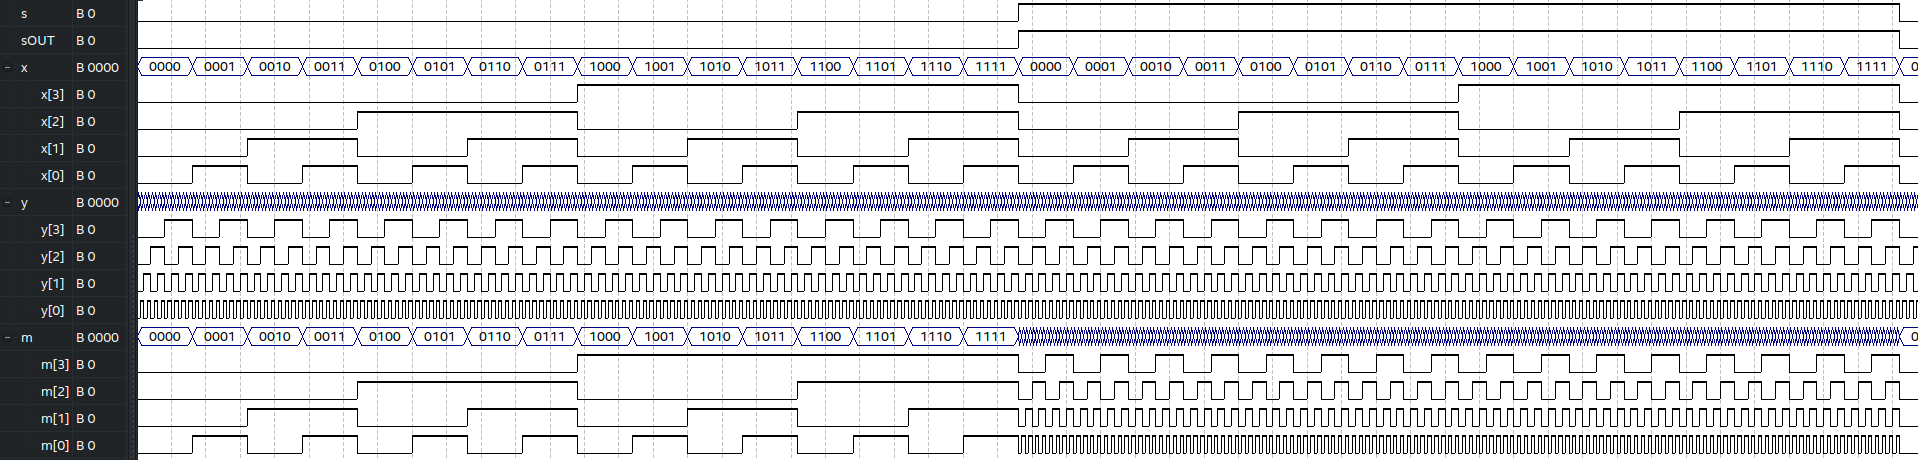
\includegraphics[scale=1.1]{images/Exc1_waveform.png}
\end{figure}

\subsection{Result of RTL viewer}
\begin{figure}[H]
\centering
\subfloat[][2-to-1 multiplexer]{
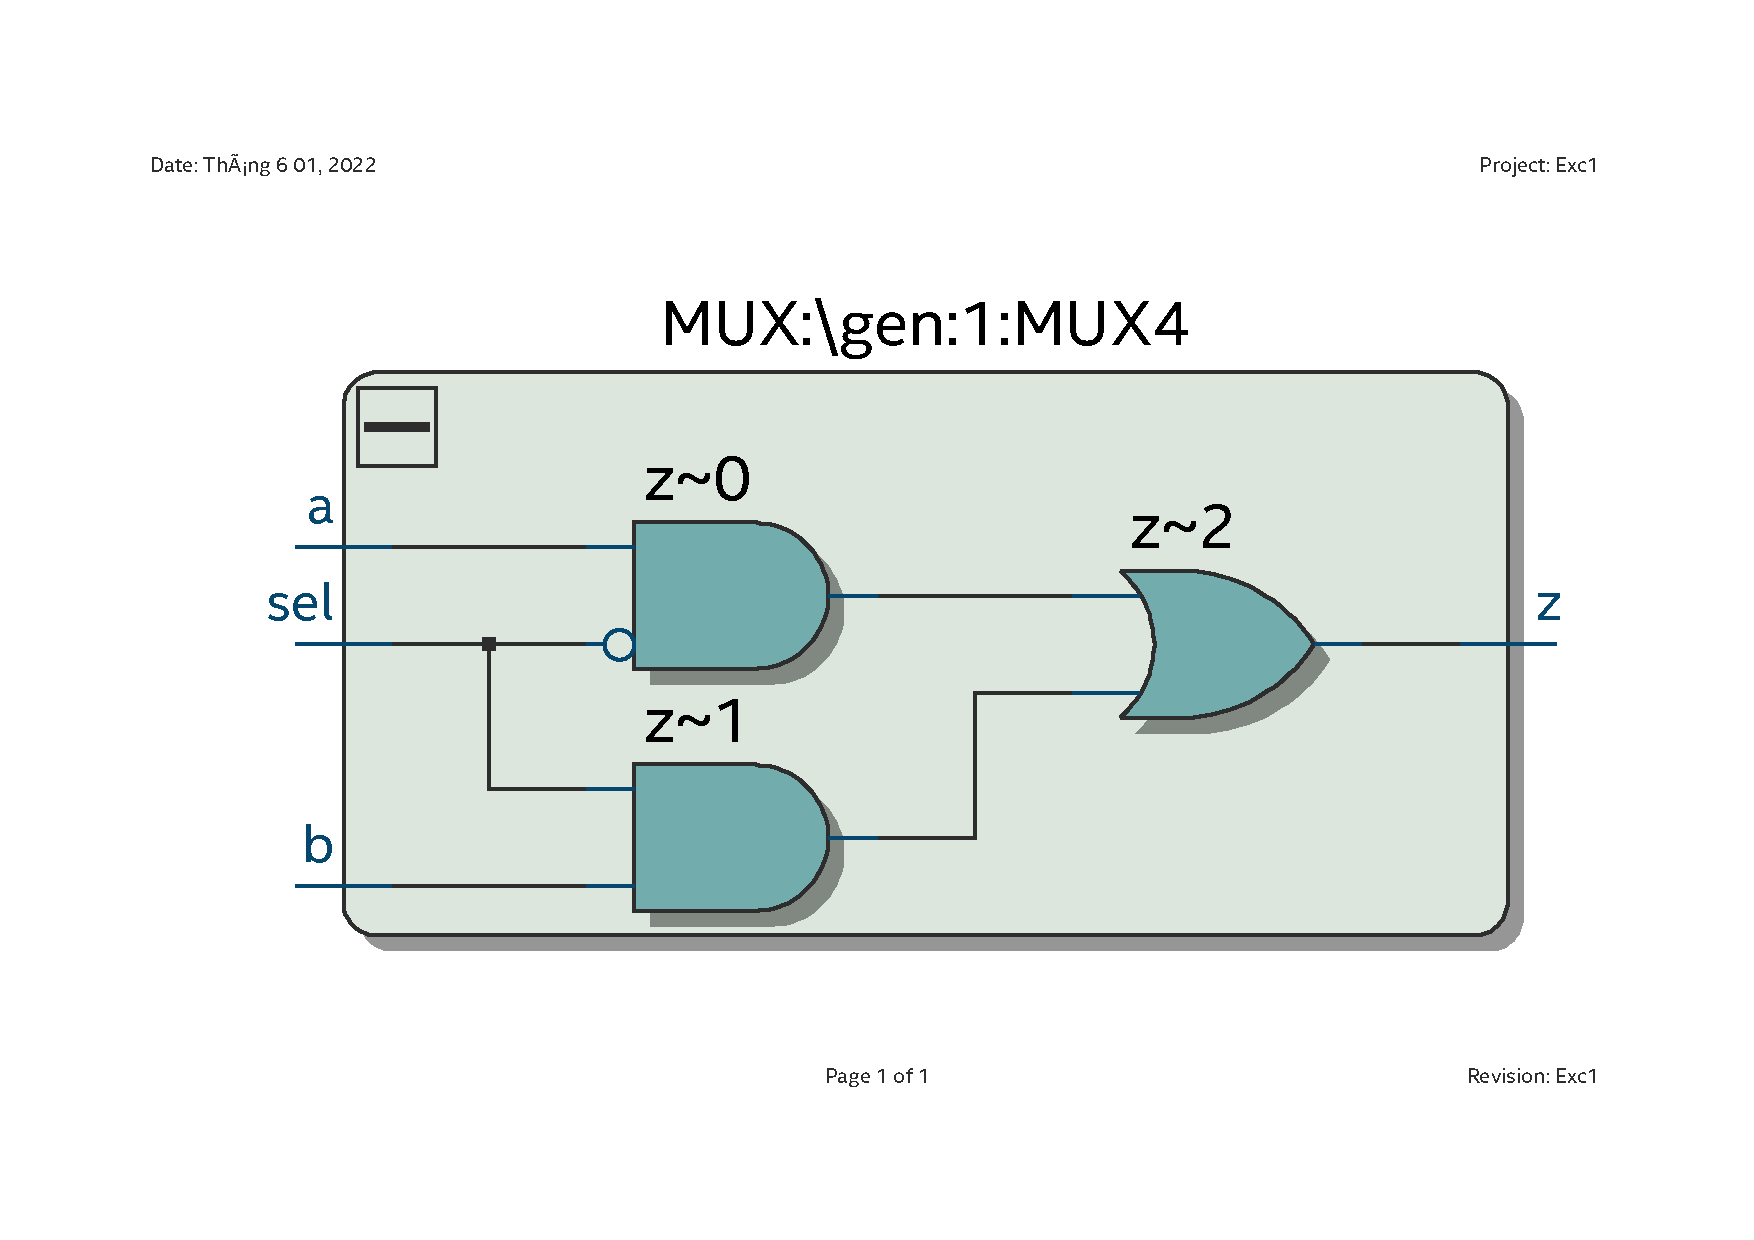
\includegraphics[scale=0.3, clip, trim={2cm 4cm 2cm 6.2cm}]{images/Exc1_MUX_RTL.pdf}}
\subfloat[][4-bit 2-to-1 multiplexer]{
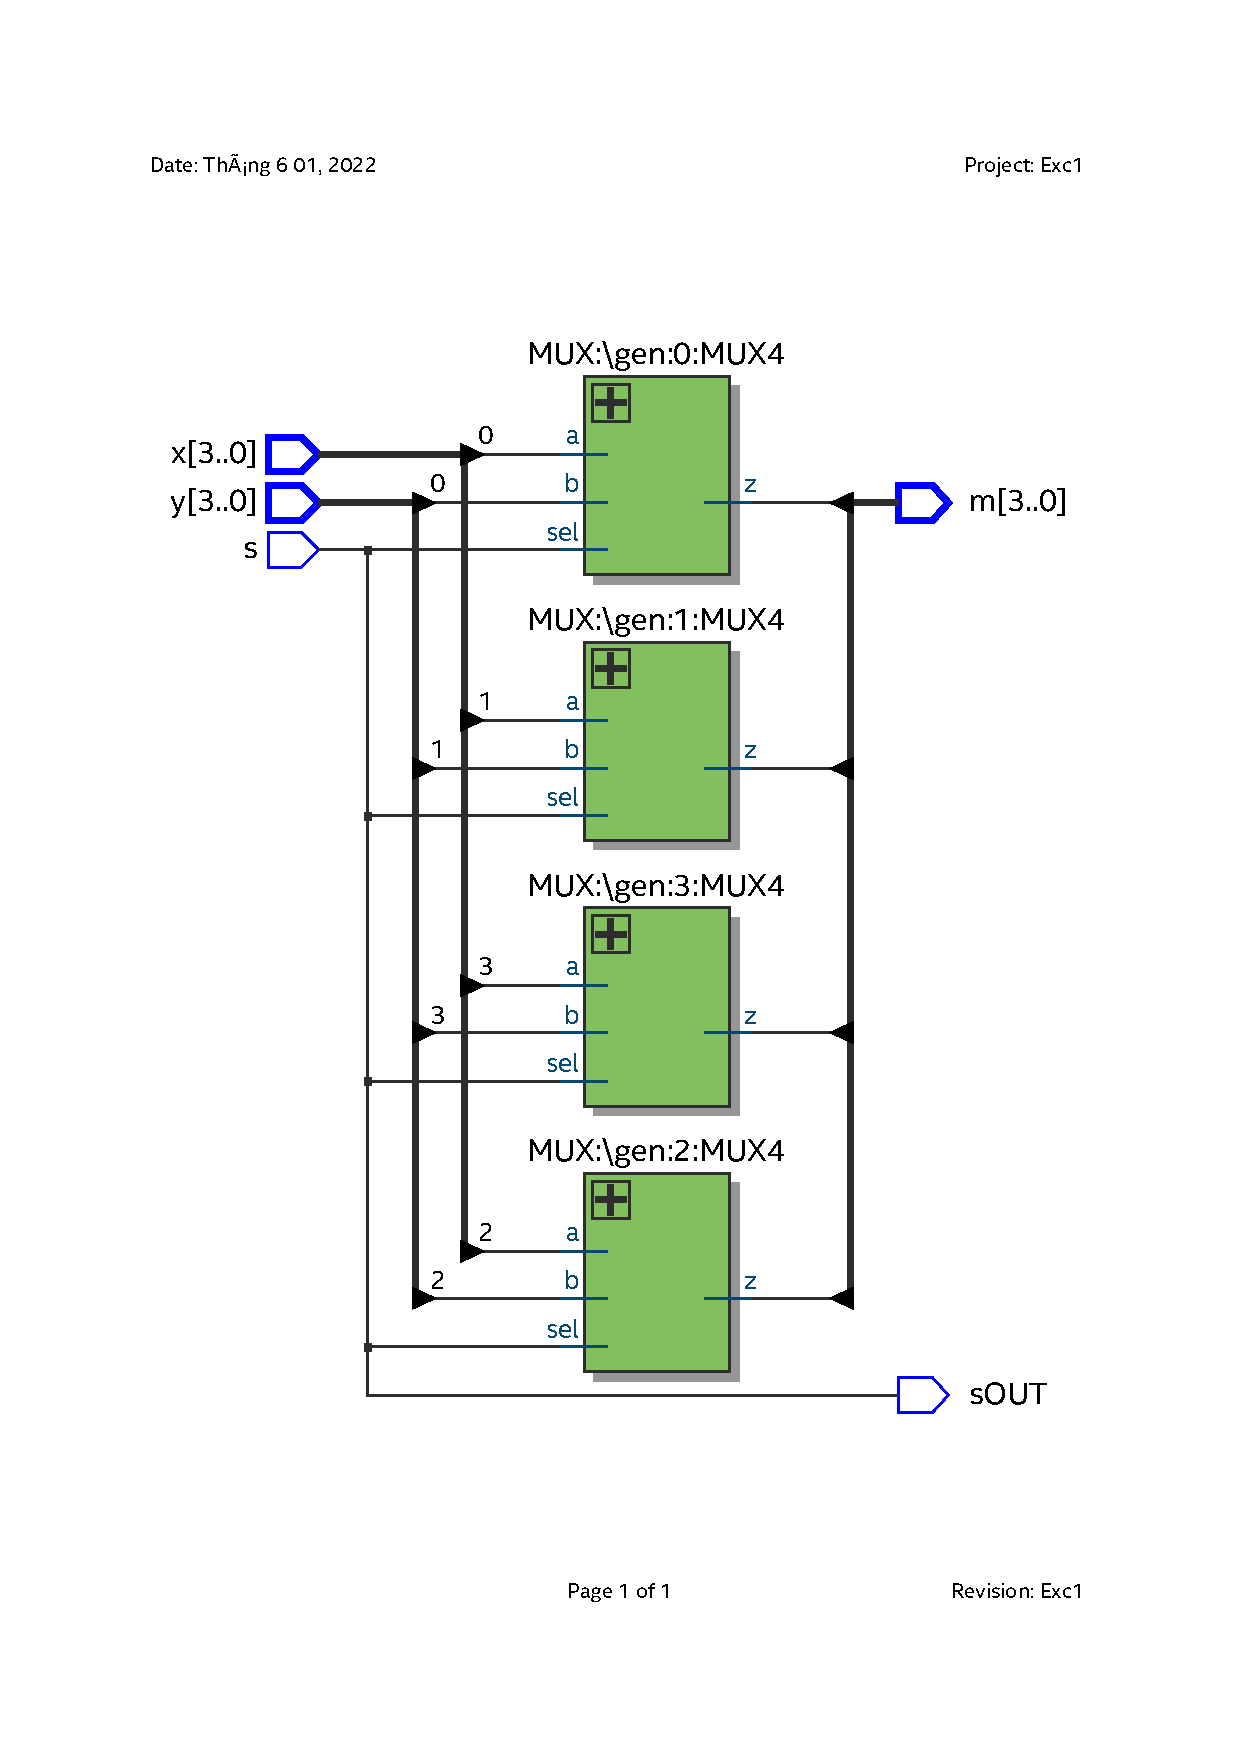
\includegraphics[scale=0.5, clip, trim={2cm 5cm 2cm 5cm}]{images/Exc1_RTL.pdf}}
\end{figure}

\section{Known how to program n-bit wide 4-to-1 multiplexer}

\begin{figure}[H]
\centering
\begin{circuitikz}
\tikzset{mux21/.style={muxdemux, muxdemux def={NL=4, NB=0, NT=2, NR=1, Lh=7, Rh=4, w=1.5}}}

\draw
  (0,0) node[mux21] (mux21) {}
  
  (mux21.lpin 1) to [multiwire=2] ++(-1,0) node[anchor=east] {$U$}
  (mux21.lpin 2) to [multiwire=2] ++(-1,0) node[anchor=east] {$V$}
  (mux21.lpin 3) to [multiwire=2] ++(-1,0) node[anchor=east] {$W$}
  (mux21.lpin 4) to [multiwire=2] ++(-1,0) node[anchor=east] {$X$}
  (mux21.rpin 1) to [multiwire=2] ++(1,0) node[anchor=west] {$M$}
  (mux21.tpin 1) -- ++(0,0.5) node[anchor=south] {$s_1$}
  (mux21.tpin 2) -- ++(0,0.5) node[anchor=south] {$s_0$}
  ;
  
\draw 
  
    ;
\end{circuitikz}
\caption*{Circuit diagram}
\end{figure}


\subsection{Code}
\subsubsection{Four2OneMUX.vhdl}
\begin{minted}{vhdl}
LIBRARY ieee;
USE ieee.std_logic_1164.ALL;

ENTITY Four2OneMUX IS
	PORT (
		s : IN std_logic_vector(1 DOWNTO 0);
		u : IN std_logic;
		v : IN std_logic;
		w : IN std_logic;
		x : IN std_logic;
		m : OUT std_logic
	);
END ENTITY;

ARCHITECTURE behave OF Four2OneMUX IS
BEGIN
	WITH s SELECT
	m <= u WHEN "00", 
	     v WHEN "01", 
	     w WHEN "10", 
	     x WHEN "11";

END ARCHITECTURE;
\end{minted}

\subsubsection{Exc1.vhdl}
\begin{minted}{vhdl}
LIBRARY ieee;
USE ieee.std_logic_1164.ALL;

ENTITY Exc2 IS
	PORT (
		ss : IN std_logic_vector(1 DOWNTO 0);
		uu : IN std_logic_vector(1 DOWNTO 0);
		vv : IN std_logic_vector(1 DOWNTO 0);
		ww : IN std_logic_vector(1 DOWNTO 0);
		xx : IN std_logic_vector(1 DOWNTO 0);
		mm : OUT std_logic_vector(1 DOWNTO 0)
	);
END ENTITY;

ARCHITECTURE behave OF Exc2 IS
	COMPONENT Four2OneMUX IS
		PORT (
			s : IN std_logic_vector(1 DOWNTO 0);
			u : IN std_logic;
			v : IN std_logic;
			w : IN std_logic;
			x : IN std_logic;
			m : OUT std_logic
		);
	END COMPONENT;

BEGIN
	gen : FOR i IN 1 DOWNTO 0 GENERATE
		MUX2 : Four2OneMUX
		PORT MAP(
			s => ss, 
			u => uu(i), 
			v => vv(i), 
			w => ww(i), 
			x => xx(i), 
			m => mm(i)
		);
	END GENERATE;

END ARCHITECTURE;
\end{minted}

\subsection{Waveform}
\begin{figure}[H]
\centering
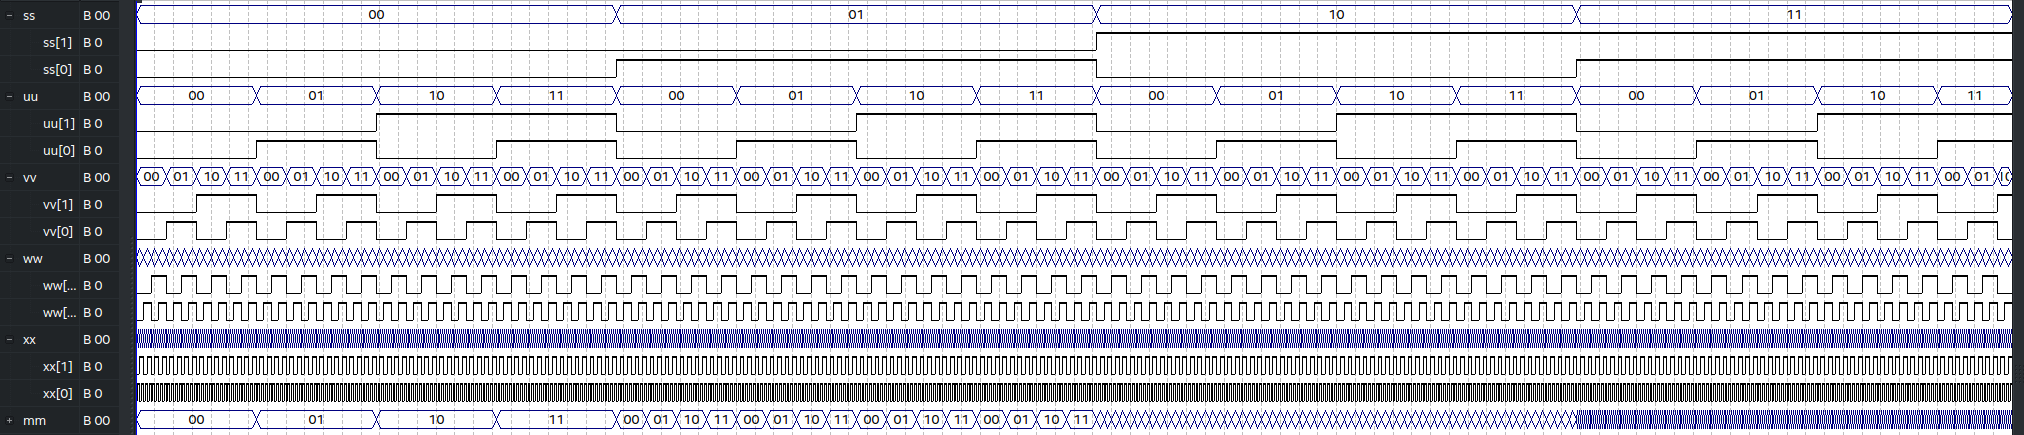
\includegraphics[scale=1.05]{images/Exc2_waveform.png}
\end{figure}

\subsection{Result of RTL viewer}
\begin{figure}[H]
\centering
\subfloat[][4-to-1 multiplexer]{
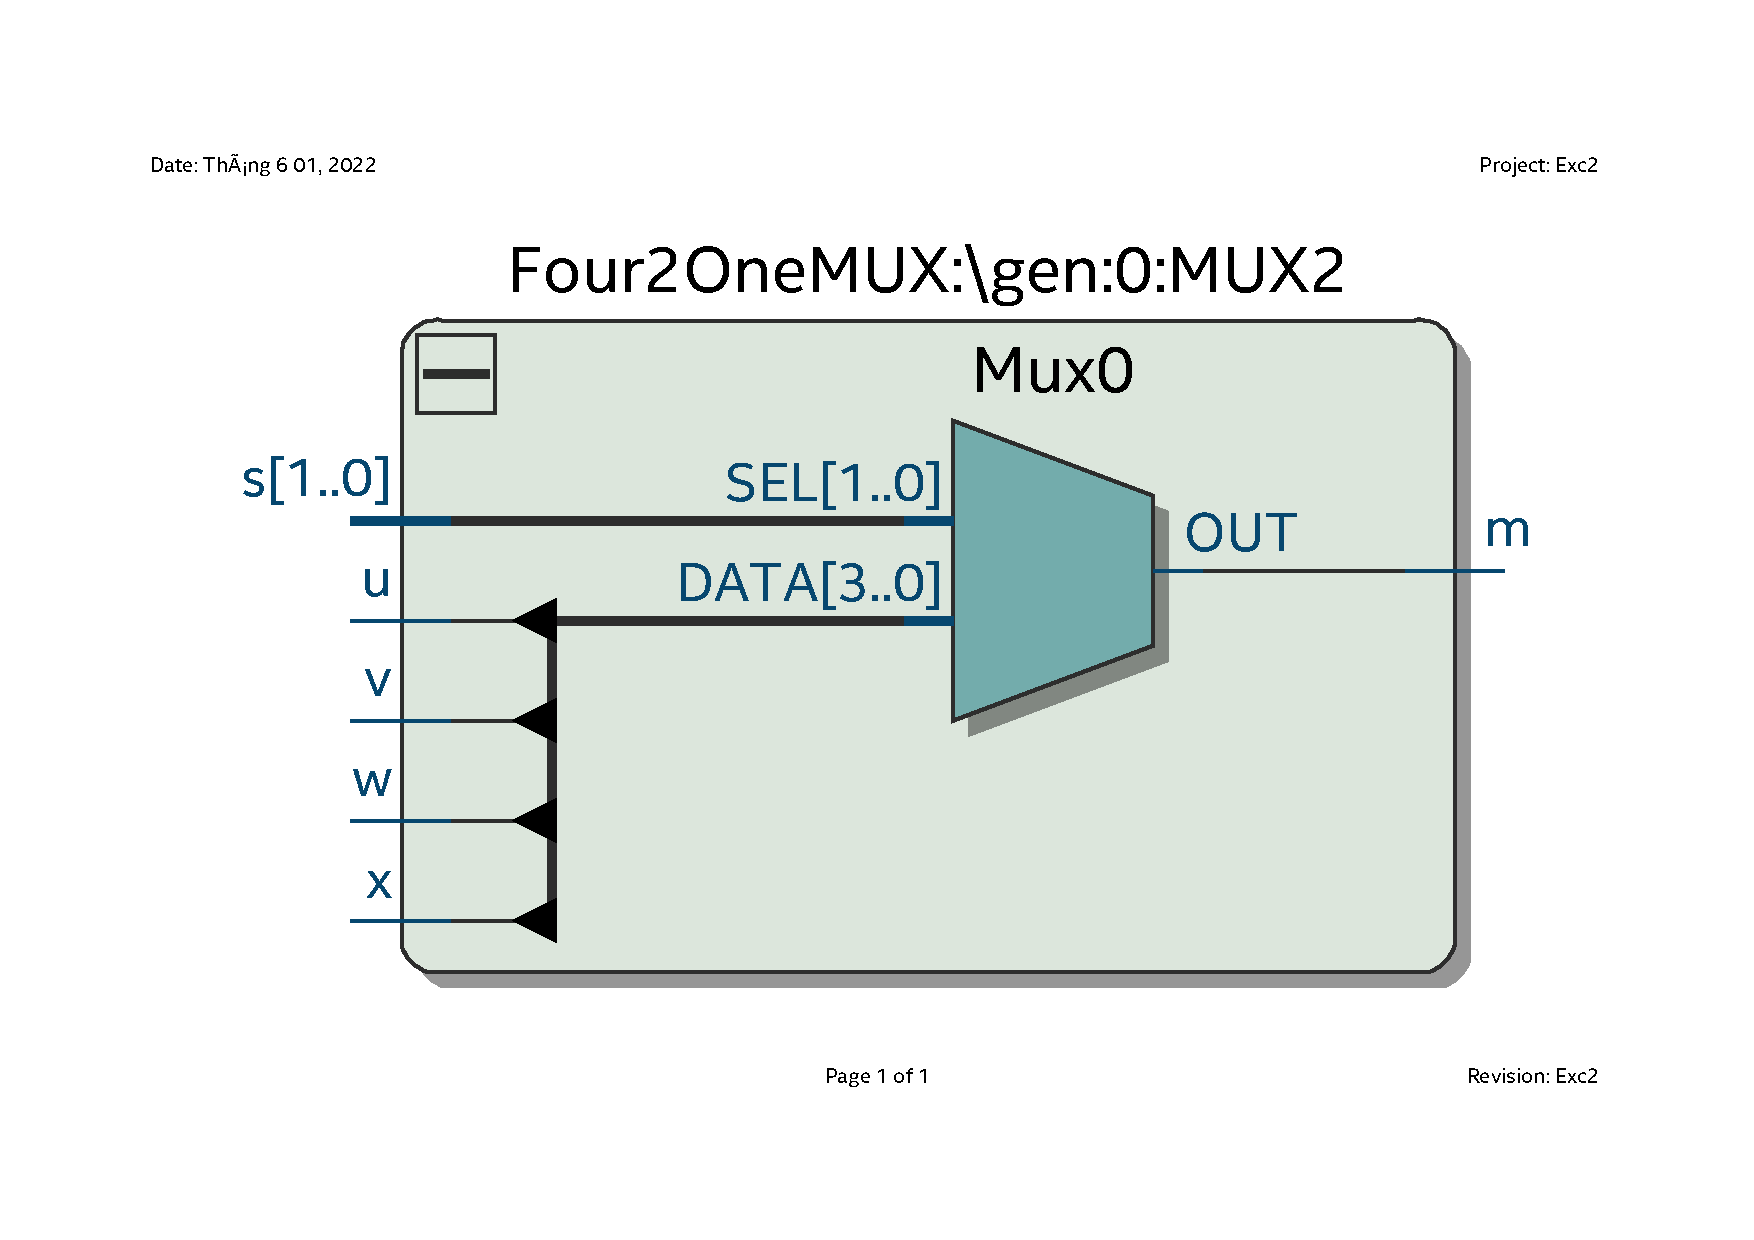
\includegraphics[scale=0.25, clip, trim={2cm 4cm 2cm 5.3cm}]{images/Exc2_MUX_RTL.pdf}}
\subfloat[][Top level]{
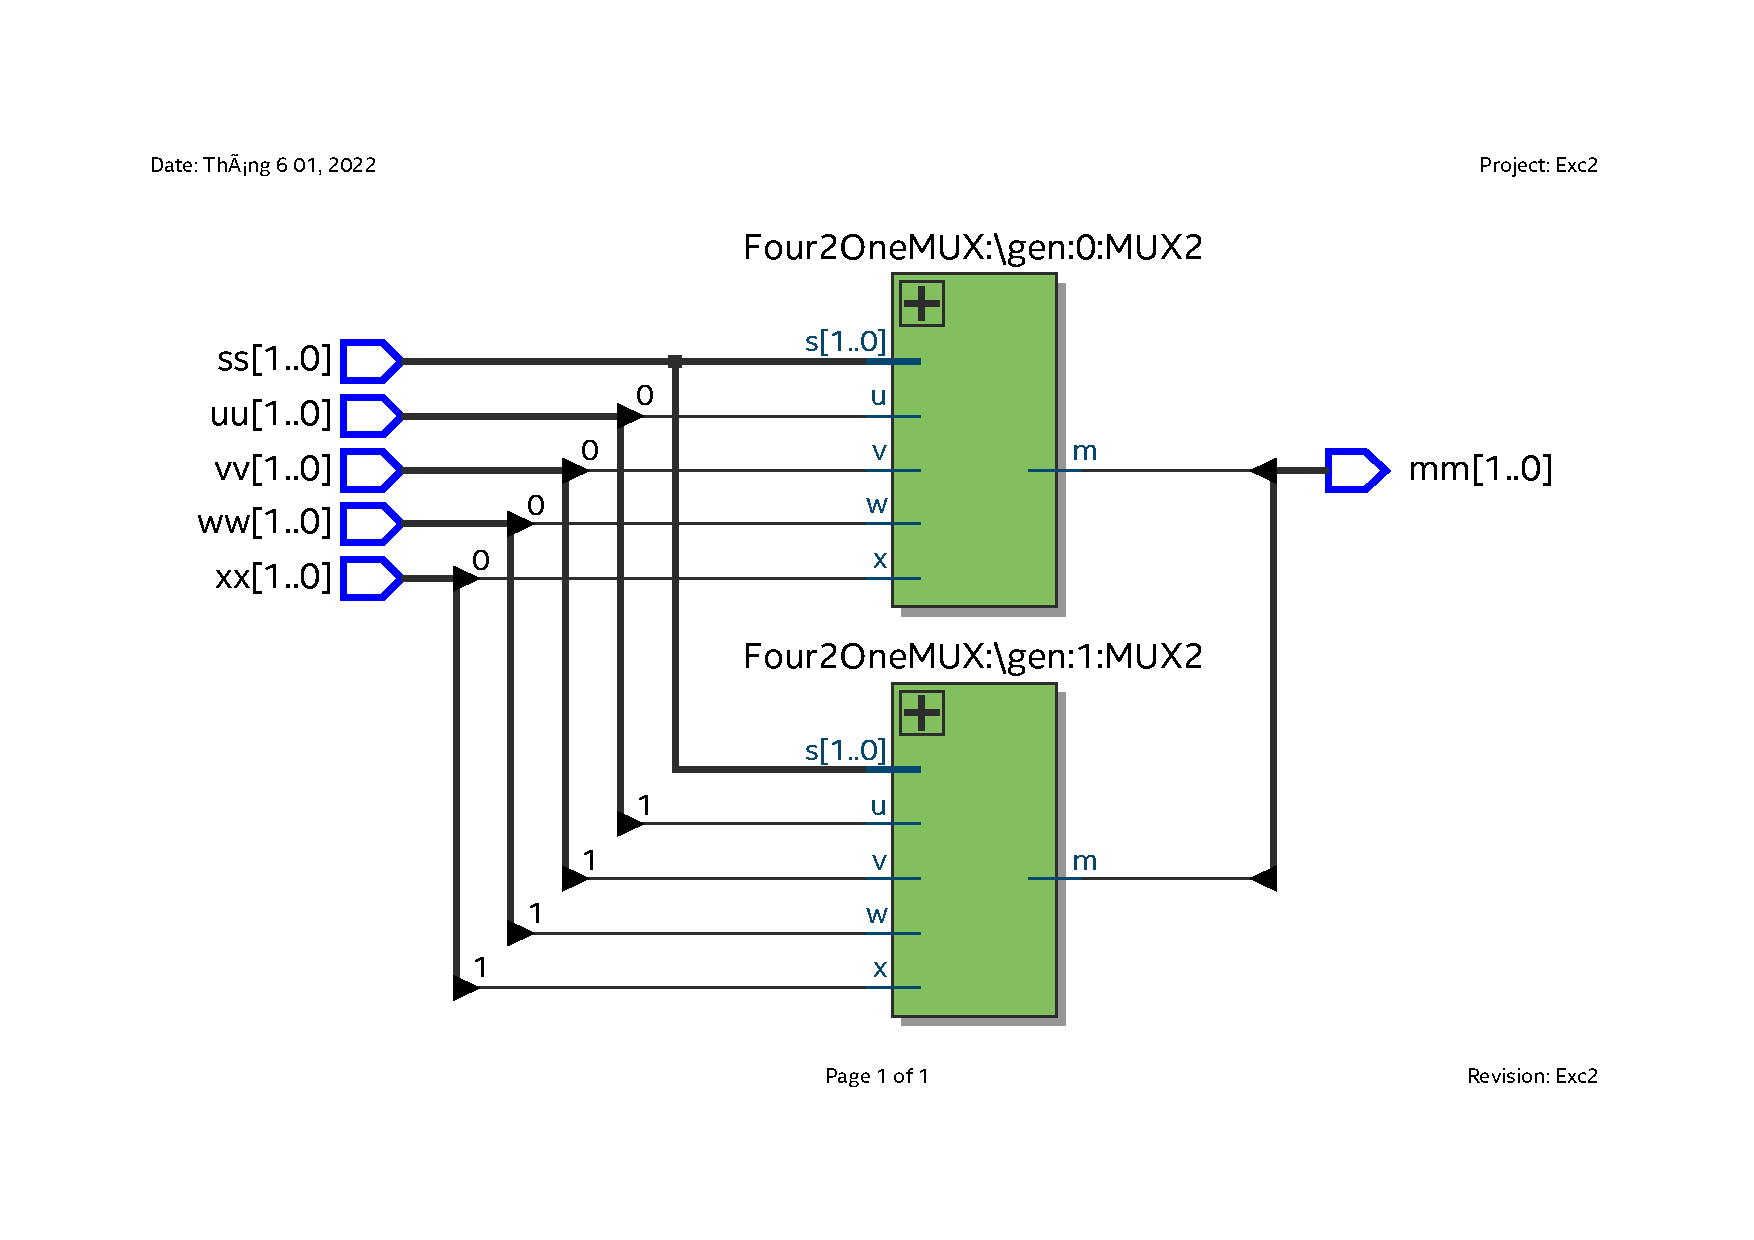
\includegraphics[scale=0.45, clip, trim={2cm 3.5cm 2cm 3.8cm}]{images/Exc2_RTL.pdf}}
\end{figure}

\section{Known how to interface with 7-segment LED}

\begin{table}[H]
\centering
\begin{tabular}{cc|c}
$s_1$ & $s_0$ & LEDs                                                                                                                                                                                                                        \\ \hline
0     & 0     & \begin{circuitikz}\ctikzset{seven seg/width=0.25, seven seg/thickness=3pt}\draw (0,0) node[seven segment val=d dot none box off]{}; \draw (1,0) node[seven segment val=E dot none box off]{}; \draw (2,0) node[seven segment val=1 dot none box off]{}; \draw (3,0) node[seven segment val=0 dot none box off]{};\end{circuitikz} \\
0     & 1     & \begin{circuitikz}\ctikzset{seven seg/width=0.25, seven seg/thickness=3pt}\draw (0,0) node[seven segment val=E dot none box off]{}; \draw (1,0) node[seven segment val=1 dot none box off]{}; \draw (2,0) node[seven segment val=0 dot none box off]{}; \draw (3,0) node[seven segment val=d dot none box off]{};\end{circuitikz} \\
1     & 0     & \begin{circuitikz}\ctikzset{seven seg/width=0.25, seven seg/thickness=3pt}\draw (0,0) node[seven segment val=1 dot none box off]{}; \draw (1,0) node[seven segment val=0 dot none box off]{}; \draw (2,0) node[seven segment val=d dot none box off]{}; \draw (3,0) node[seven segment val=E dot none box off]{};\end{circuitikz} \\
1     & 1     & \begin{circuitikz}\ctikzset{seven seg/width=0.25, seven seg/thickness=3pt}\draw (0,0) node[seven segment val=0 dot none box off]{}; \draw (1,0) node[seven segment val=d dot none box off]{}; \draw (2,0) node[seven segment val=E dot none box off]{}; \draw (3,0) node[seven segment val=1 dot none box off]{};\end{circuitikz}
\end{tabular}
\end{table}

\subsection{Method 1: with MUX}
\subsubsection{Code}
\paragraph{DE10.vhdl}
\begin{minted}{vhdl}
LIBRARY ieee;
USE ieee.std_logic_1164.ALL;

ENTITY DE10 IS
	PORT (
		c : IN std_logic_vector(1 DOWNTO 0);
		HEXn : OUT std_logic_vector(0 TO 6)
	);
END DE10;

ARCHITECTURE behavior OF DE10 IS
	SIGNAL HEX : std_logic_vector(0 TO 6);
BEGIN
	HEXn <= NOT(HEX);
	WITH c SELECT
	HEX <= "0111101" WHEN "00", 
	       "1001111" WHEN "01", 
	       "0110000" WHEN "10", 
	       "1111110" WHEN "11", 
	       "0000000" WHEN OTHERS;
END behavior;
\end{minted}

\paragraph{Four2OneMUX.vhdl}
\begin{minted}{vhdl}
LIBRARY ieee;
USE ieee.std_logic_1164.ALL;

ENTITY Four2OneMUX IS
	PORT (
		s : IN std_logic_vector(1 DOWNTO 0);
		u : IN std_logic;
		v : IN std_logic;
		w : IN std_logic;
		x : IN std_logic;
		m : OUT std_logic
	);
END ENTITY;

ARCHITECTURE behave OF Four2OneMUX IS
BEGIN
	WITH s SELECT
	m <= u WHEN "00", 
	     v WHEN "01", 
	     w WHEN "10", 
	     x WHEN "11";

END ARCHITECTURE;
\end{minted}

\paragraph{TwoBitFour2OneMUX.vhdl}
\begin{minted}{vhdl}
LIBRARY ieee;
USE ieee.std_logic_1164.ALL;

ENTITY TwoBitFour2OneMUX IS
	PORT (
		ss : IN std_logic_vector(1 DOWNTO 0);
		uu : IN std_logic_vector(1 DOWNTO 0);
		vv : IN std_logic_vector(1 DOWNTO 0);
		ww : IN std_logic_vector(1 DOWNTO 0);
		xx : IN std_logic_vector(1 DOWNTO 0);
		mm : OUT std_logic_vector(1 DOWNTO 0)
	);
END ENTITY;

ARCHITECTURE behave OF TwoBitFour2OneMUX IS
	COMPONENT Four2OneMUX IS
		PORT (
			s : IN std_logic_vector(1 DOWNTO 0);
			u : IN std_logic;
			v : IN std_logic;
			w : IN std_logic;
			x : IN std_logic;
			m : OUT std_logic
		);
	END COMPONENT;

BEGIN
	gen : FOR i IN 1 DOWNTO 0 GENERATE
		MUX2 : Four2OneMUX
		PORT MAP(
			s => ss, 
			u => uu(i), 
			v => vv(i), 
			w => ww(i), 
			x => xx(i), 
			m => mm(i)
		);
	END GENERATE;

END ARCHITECTURE;
\end{minted}

\paragraph{Exc1.vhdl}
\begin{minted}{vhdl}
LIBRARY ieee;
USE ieee.std_logic_1164.ALL;

ENTITY Exc3 IS
	PORT (
		SW : IN std_logic_vector(9 DOWNTO 0);
		HEX0 : OUT std_logic_vector(0 TO 6);
		HEX1 : OUT std_logic_vector(0 TO 6);
		HEX2 : OUT std_logic_vector(0 TO 6);
		HEX3 : OUT std_logic_vector(0 TO 6)
	);
END ENTITY;

ARCHITECTURE behave OF Exc3 IS
	SIGNAL sel3, sel2, sel1, sel0, selct : std_logic_vector(1 DOWNTO 0);
	SIGNAL outHEX3, outHEX2, outHEX1, outHEX0 : std_logic_vector(1 DOWNTO 0);
 
	COMPONENT DE10 IS
		PORT (
			c : IN std_logic_vector(1 DOWNTO 0);
			HEXn : OUT std_logic_vector(0 TO 6)
		);
	END COMPONENT;
 
	COMPONENT TwoBitFour2OneMUX IS
		PORT (
			ss : IN std_logic_vector(1 DOWNTO 0);
			uu : IN std_logic_vector(1 DOWNTO 0);
			vv : IN std_logic_vector(1 DOWNTO 0);
			ww : IN std_logic_vector(1 DOWNTO 0);
			xx : IN std_logic_vector(1 DOWNTO 0);
			mm : OUT std_logic_vector(1 DOWNTO 0)
		);
	END COMPONENT;

BEGIN
	selct <= SW(9 DOWNTO 8);
	sel3 <= SW(7 DOWNTO 6);
	sel2 <= SW(5 DOWNTO 4);
	sel1 <= SW(3 DOWNTO 2);
	sel0 <= SW(1 DOWNTO 0);
	MUX3 : TwoBitFour2OneMUX
	PORT MAP(
		uu => sel3, vv => sel2, ww => sel1, xx => sel0, ss => selct, mm => outHEX3
	);
	MUX2 : TwoBitFour2OneMUX
	PORT MAP(
		uu => sel2, vv => sel1, ww => sel0, xx => sel3, ss => selct, mm => outHEX2
	);
	MUX1 : TwoBitFour2OneMUX
	PORT MAP(
		uu => sel1, vv => sel0, ww => sel3, xx => sel2, ss => selct, mm => outHEX1
	);
	MUX0 : TwoBitFour2OneMUX
	PORT MAP(
		uu => sel0, vv => sel3, ww => sel2, xx => sel1, ss => selct, mm => outHEX0
	);
 
	HEX03 : DE10
	PORT MAP(c => outHEX3, HEXn => HEX3);
	HEX02 : DE10
	PORT MAP(c => outHEX2, HEXn => HEX2);
	HEX01 : DE10
	PORT MAP(c => outHEX1, HEXn => HEX1);
HEX00 : DE10
PORT MAP(c => outHEX0, HEXn => HEX0);
 
END ARCHITECTURE;
\end{minted}

\subsubsection{Result of RTL viewer}
\begin{figure}[H]
\centering
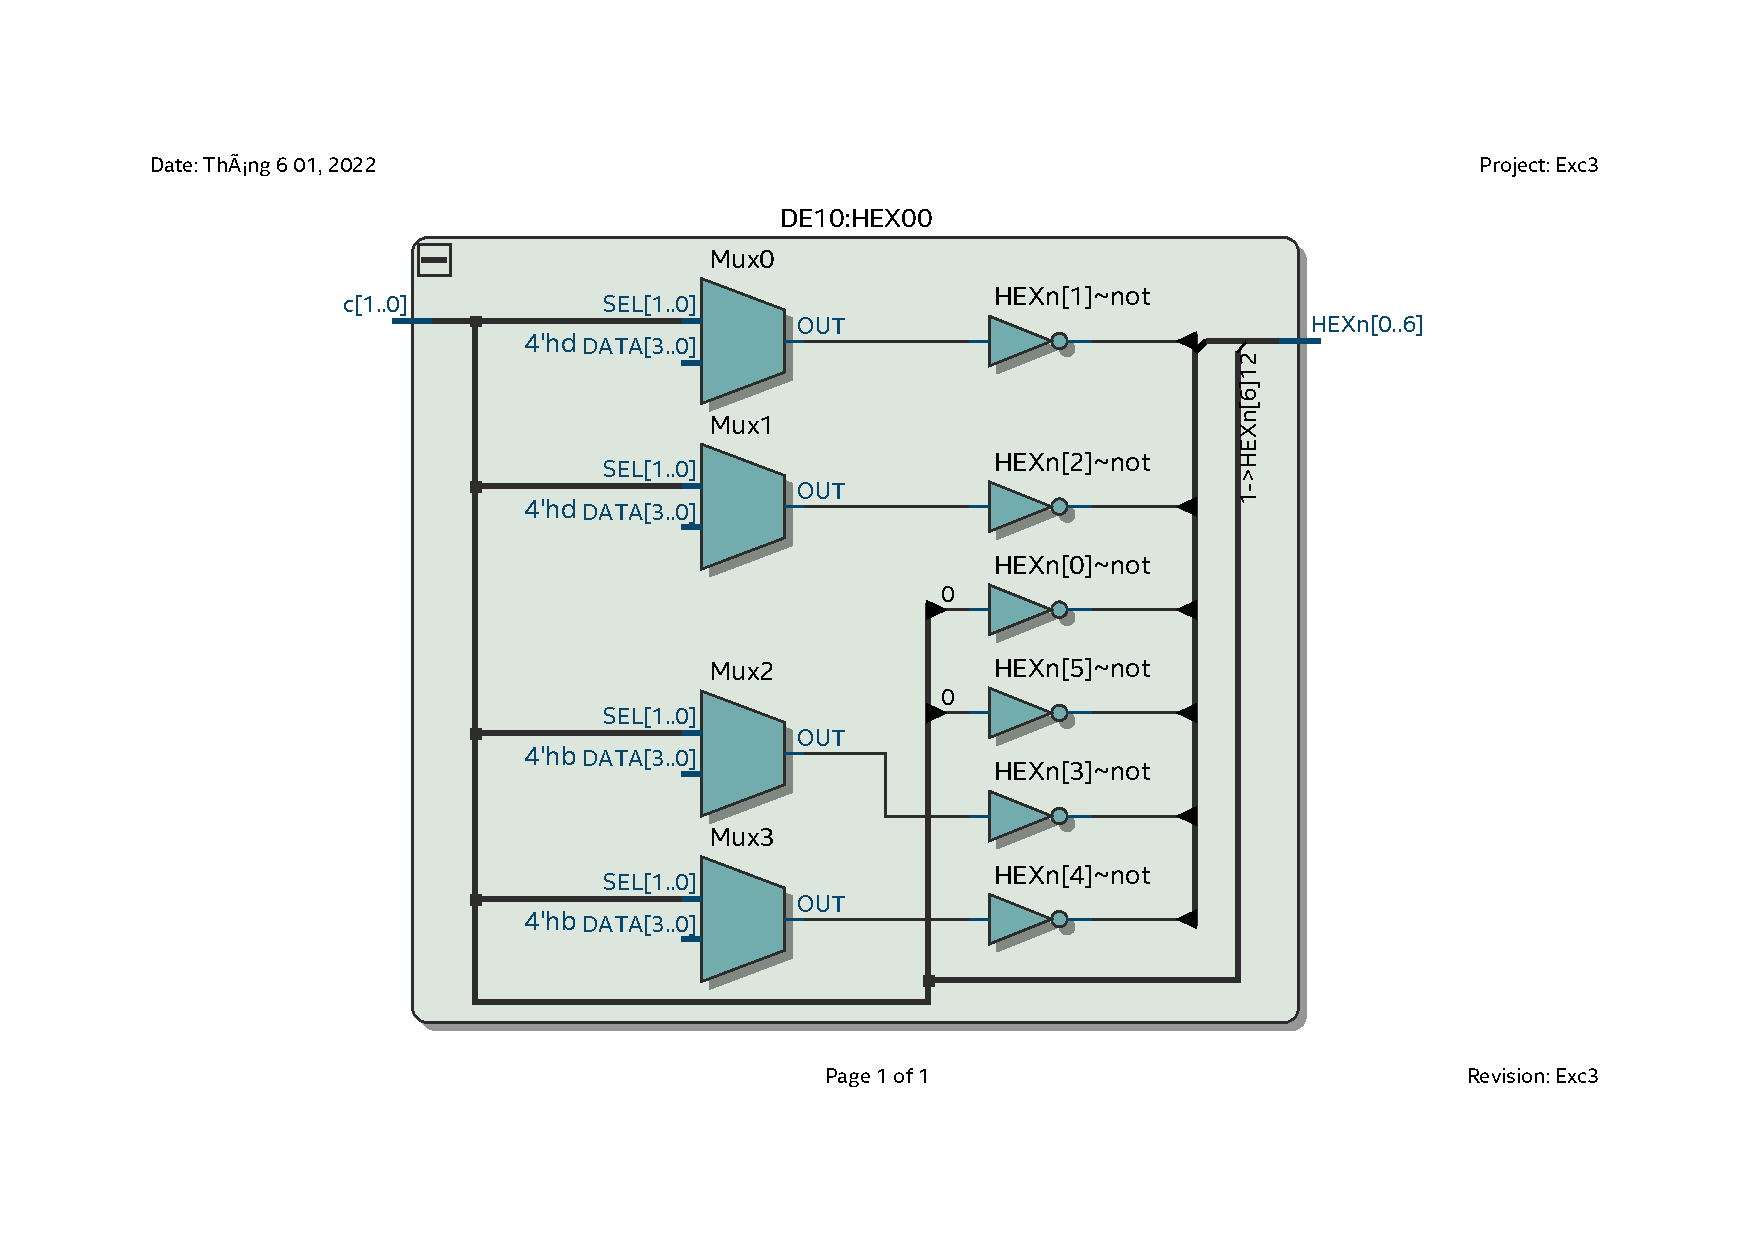
\includegraphics[scale=0.7, clip, trim={2cm 3.5cm 2cm 4cm}]{images/Exc3_HEX_RTL.pdf}
\caption*{"dE10" 7-segment decoder}
\end{figure}

\begin{figure}[H]
\centering
\subfloat[][4-to-1 multiplexer]{
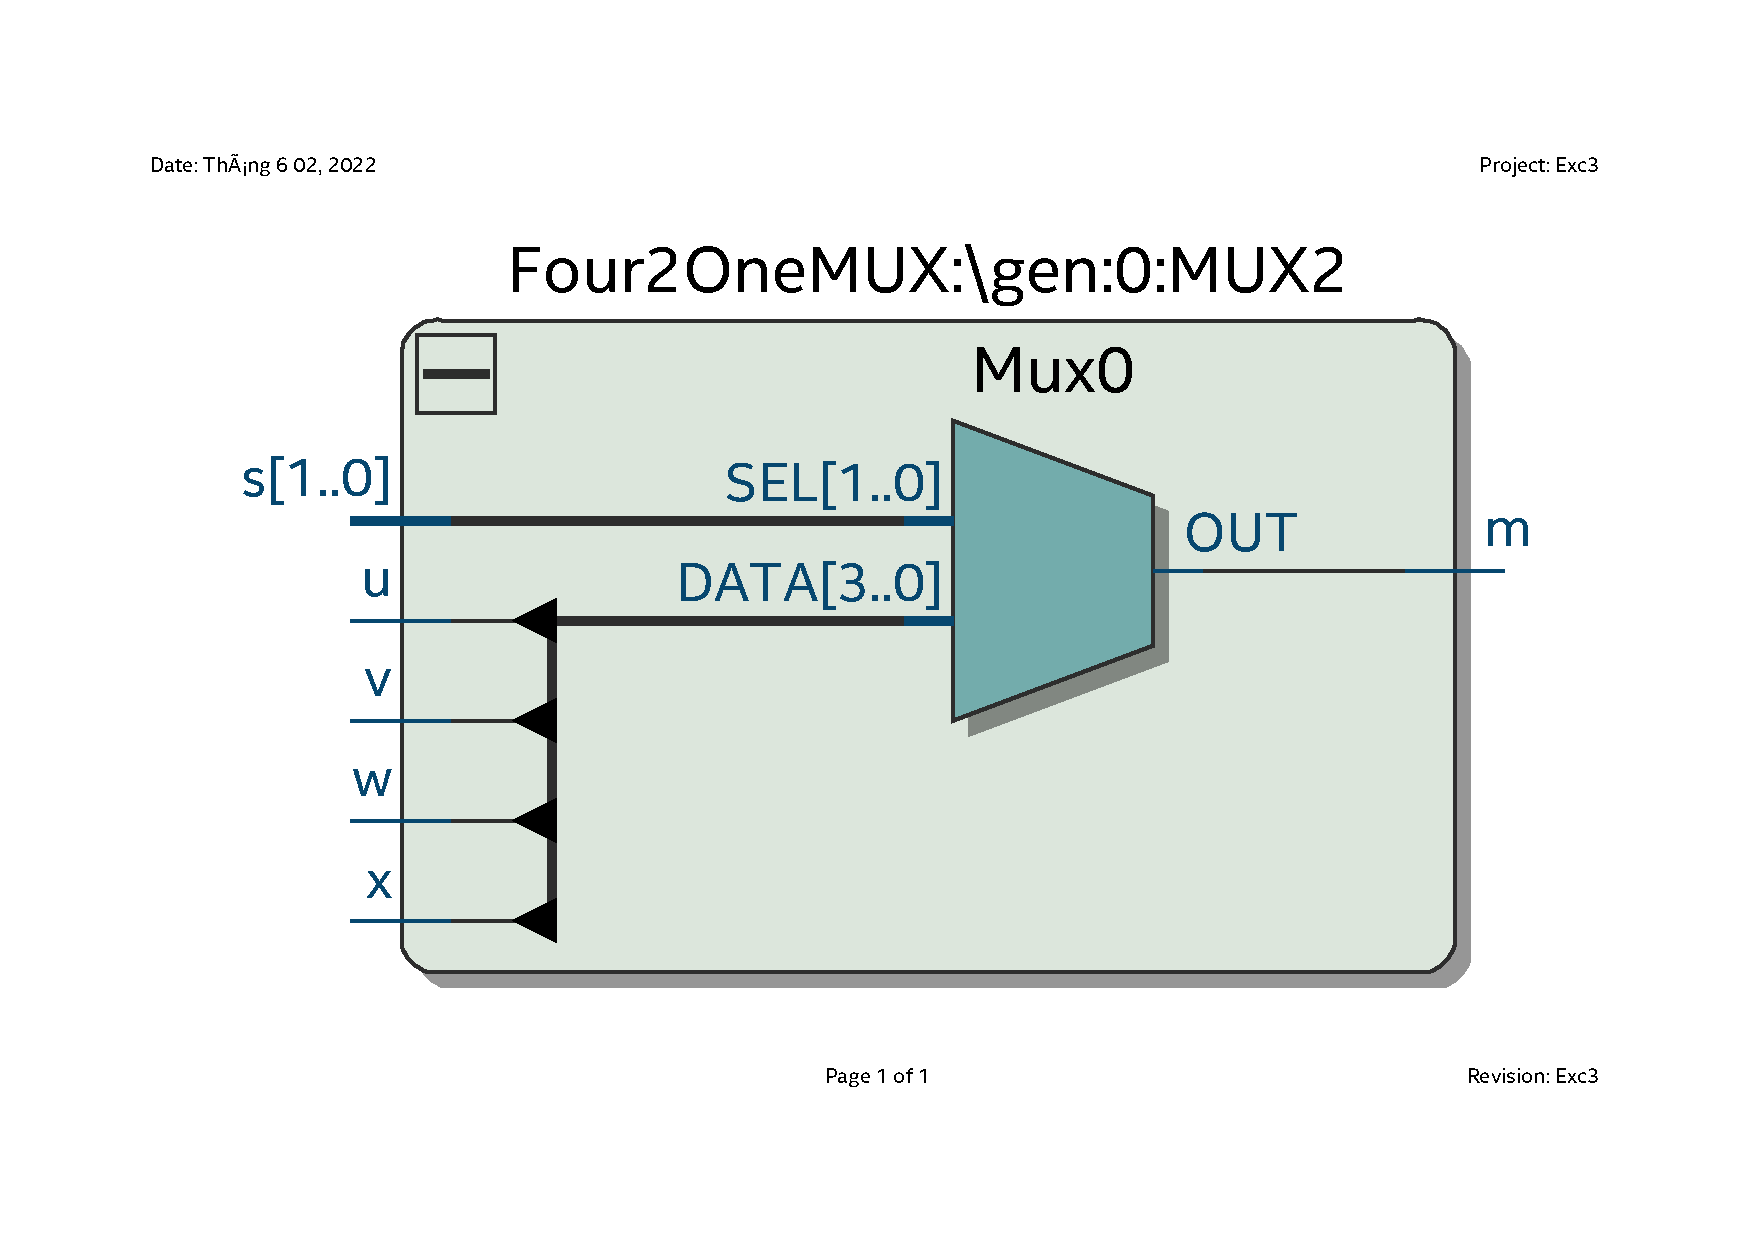
\includegraphics[scale=0.3, clip, trim={3cm 3.5cm 3cm 5.3cm}]{images/Exc3_421MUX_RTL.pdf}}
\subfloat[][2-bit 4-to-1 multiplexer]{
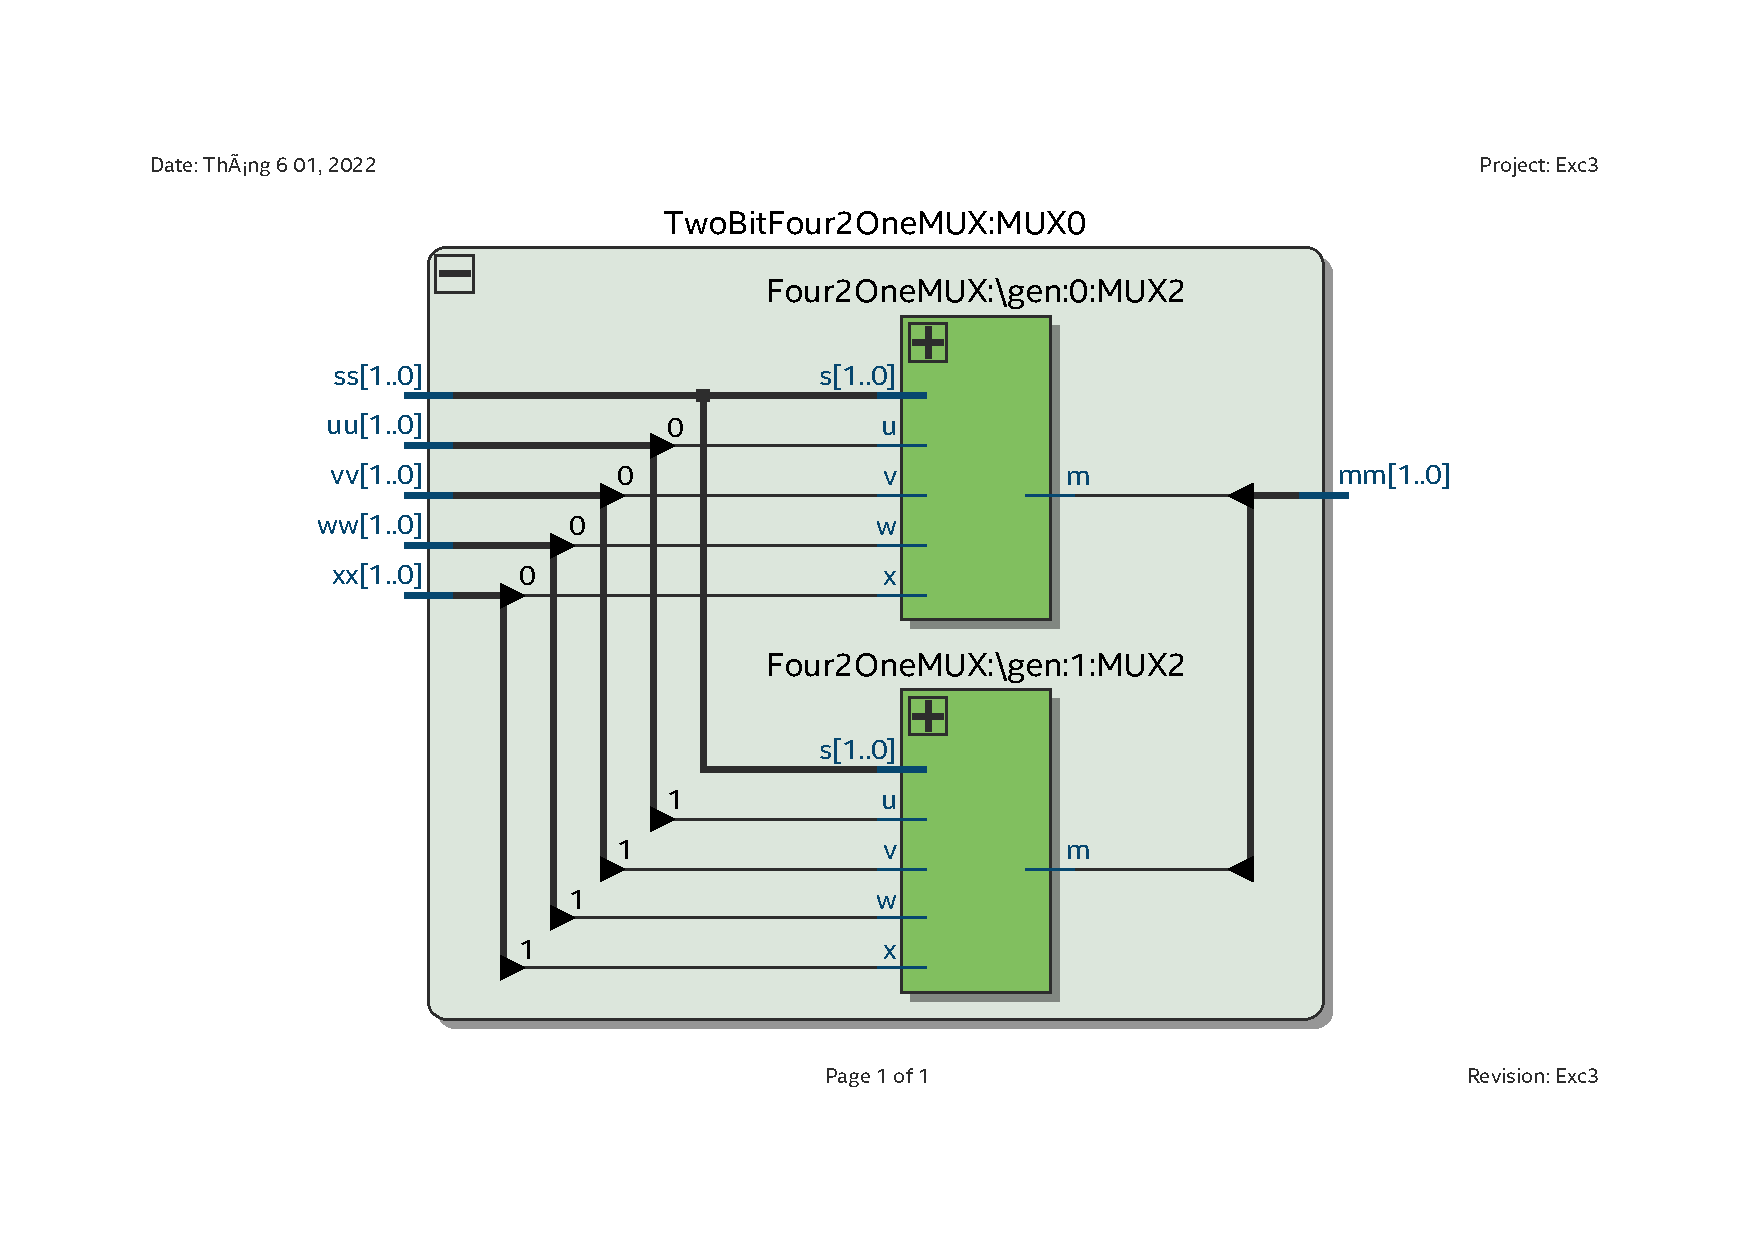
\includegraphics[scale=0.5, clip, trim={3cm 3.5cm 3cm 4.2cm}]{images/Exc3_MUX_RTL.pdf}}
\end{figure}

\begin{figure}[H]
\centering
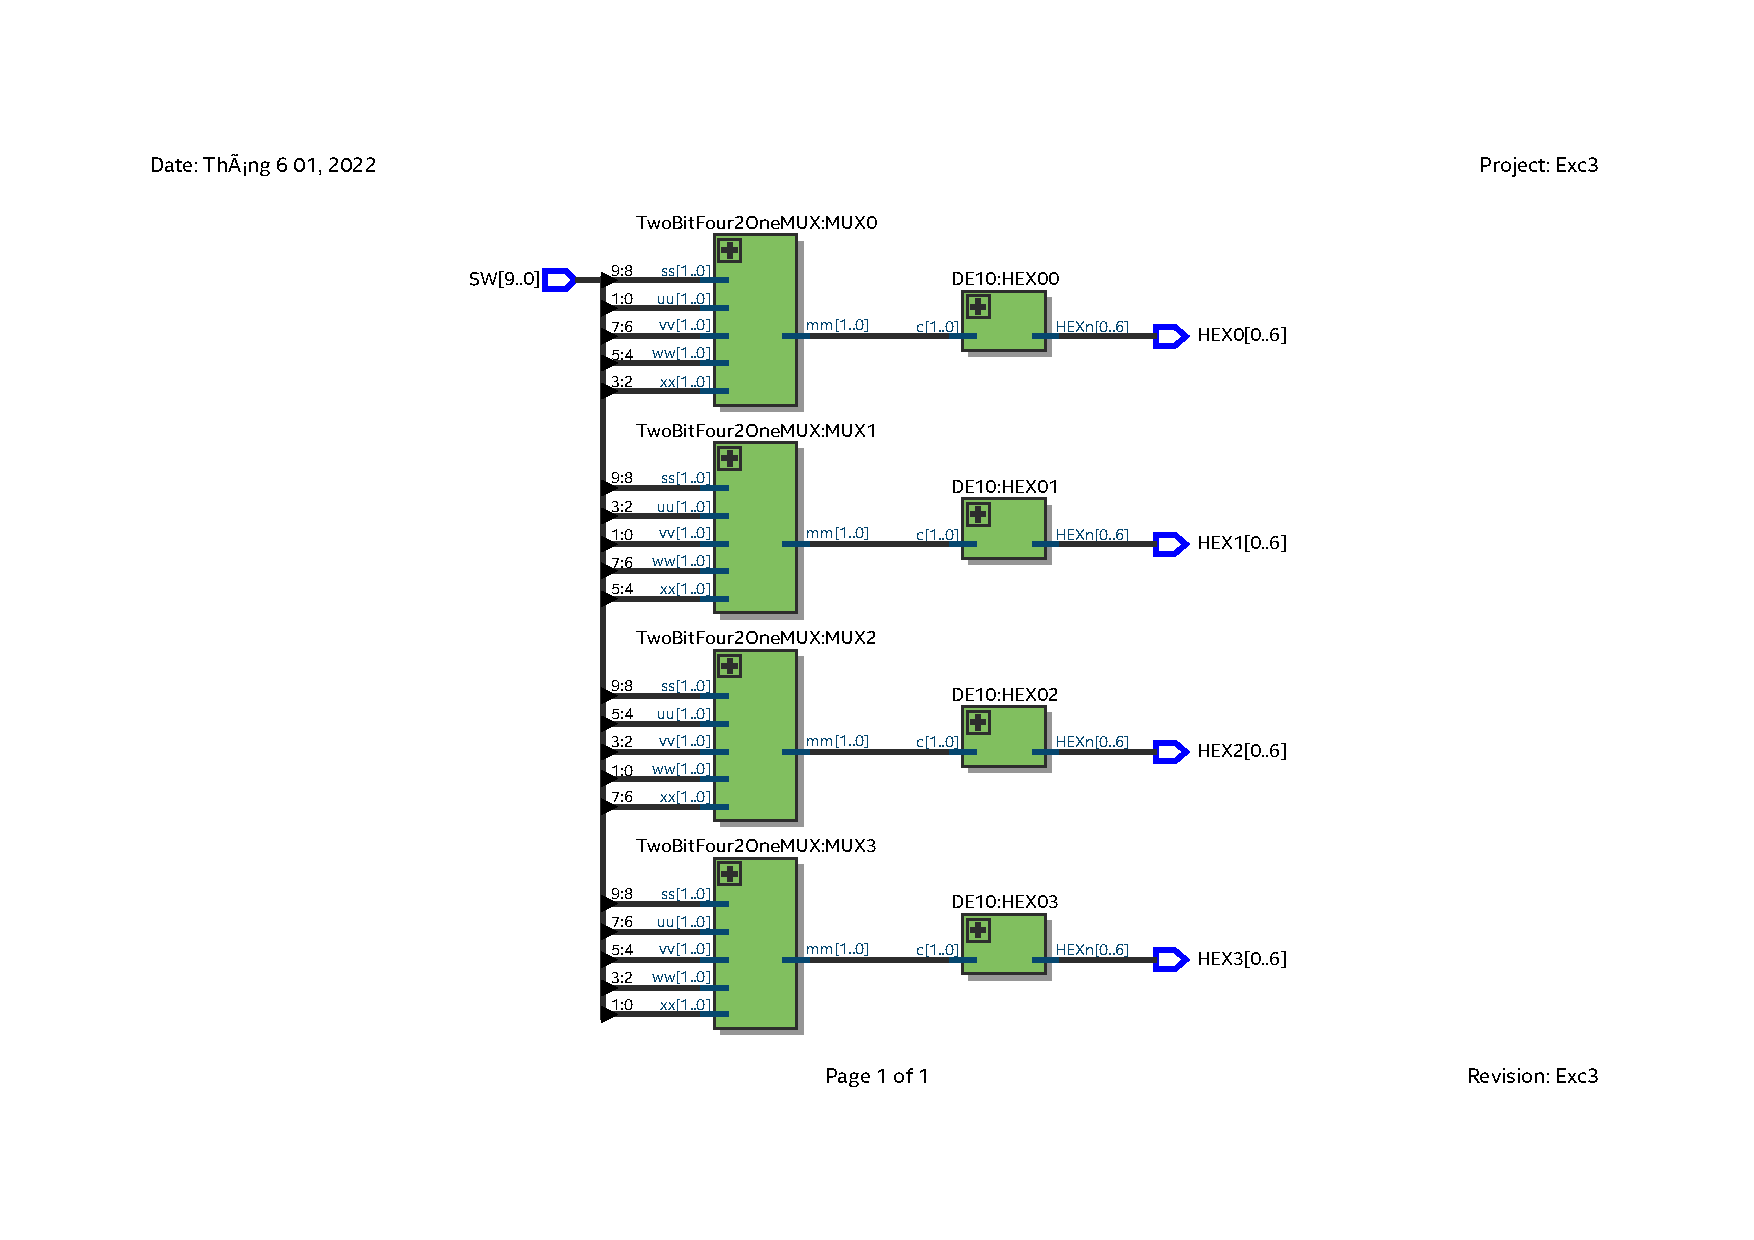
\includegraphics[scale=0.9, clip, trim={4cm 3.5cm 3cm 3.5cm}]{images/Exc3_RTL_1.pdf}
\caption*{Top level}
\end{figure}

\subsection{Method 2: without MUX}
\subsubsection{Code}
\paragraph{DE10.vhdl}
\begin{minted}{vhdl}
LIBRARY ieee;
USE ieee.std_logic_1164.ALL;

ENTITY DE10 IS
	PORT (
		c : IN std_logic_vector(1 DOWNTO 0);
		HEXn : OUT std_logic_vector(0 TO 6)
	);
END DE10;

ARCHITECTURE behavior OF DE10 IS
	SIGNAL HEX : std_logic_vector(0 TO 6);
BEGIN
	HEXn <= NOT(HEX);
	WITH c SELECT
	HEX <= "0111101" WHEN "00", 
	       "1001111" WHEN "01", 
	       "0110000" WHEN "10", 
	       "1111110" WHEN "11", 
	       "0000000" WHEN OTHERS;
END behavior;
\end{minted}

\paragraph{Exc1.vhdl}
\begin{minted}{vhdl}
LIBRARY ieee;
USE ieee.std_logic_1164.ALL;
USE IEEE.numeric_std.ALL;

ENTITY Exc3 IS
	PORT (
		SW : IN std_logic_vector(9 DOWNTO 0);
		HEX0 : OUT std_logic_vector(0 TO 6);
		HEX1 : OUT std_logic_vector(0 TO 6);
		HEX2 : OUT std_logic_vector(0 TO 6);
		HEX3 : OUT std_logic_vector(0 TO 6)
	);
END ENTITY;

ARCHITECTURE behave OF Exc3 IS
	SIGNAL sel3, sel2, sel1, sel0 : std_logic_vector(1 DOWNTO 0);
 
	COMPONENT DE10 IS
		PORT (
			c : IN std_logic_vector(1 DOWNTO 0);
			HEXn : OUT std_logic_vector(0 TO 6)
		);
	END COMPONENT;

BEGIN
	sel3 <= std_logic_vector(unsigned(SW(7 DOWNTO 6)) + unsigned(SW(9 DOWNTO 8)));
	sel2 <= std_logic_vector(unsigned(SW(5 DOWNTO 4)) + unsigned(SW(9 DOWNTO 8)));
	sel1 <= std_logic_vector(unsigned(SW(3 DOWNTO 2)) + unsigned(SW(9 DOWNTO 8)));
	sel0 <= std_logic_vector(unsigned(SW(1 DOWNTO 0)) + unsigned(SW(9 DOWNTO 8)));
 
	HEX03 : DE10 PORT MAP(c => sel3, HEXn => HEX3);
	HEX02 : DE10 PORT MAP(c => sel2, HEXn => HEX2);
	HEX01 : DE10 PORT MAP(c => sel1, HEXn => HEX1);
	HEX00 : DE10 PORT MAP(c => sel0, HEXn => HEX0);

END ARCHITECTURE;
\end{minted}


\subsubsection{Result of RTL viewer}
\begin{figure}[H]
\centering
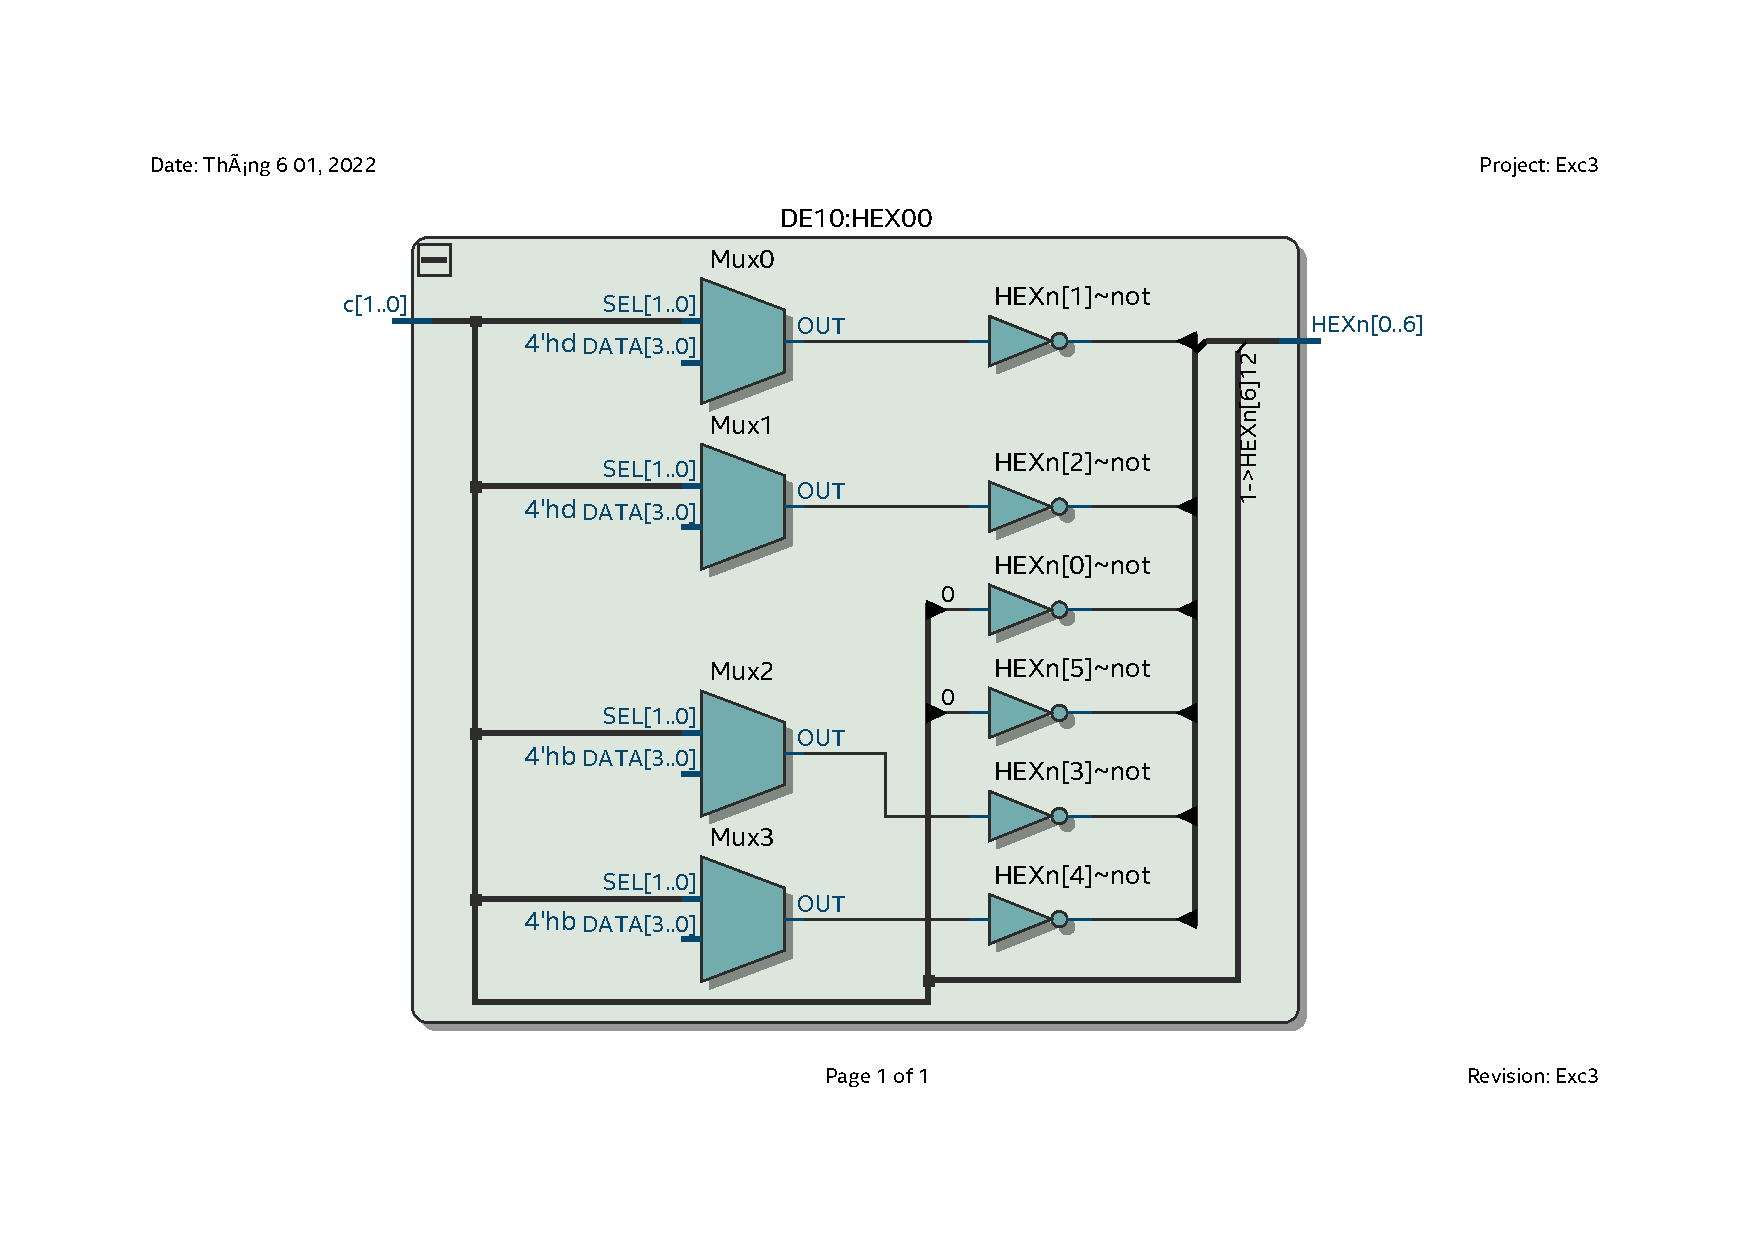
\includegraphics[scale=0.5, clip, trim={2cm 3.5cm 2cm 4cm}]{images/Exc3_HEX_RTL.pdf}
\caption*{``dE10'' 7-segment decoder}
\end{figure}

\begin{figure}[H]
\centering
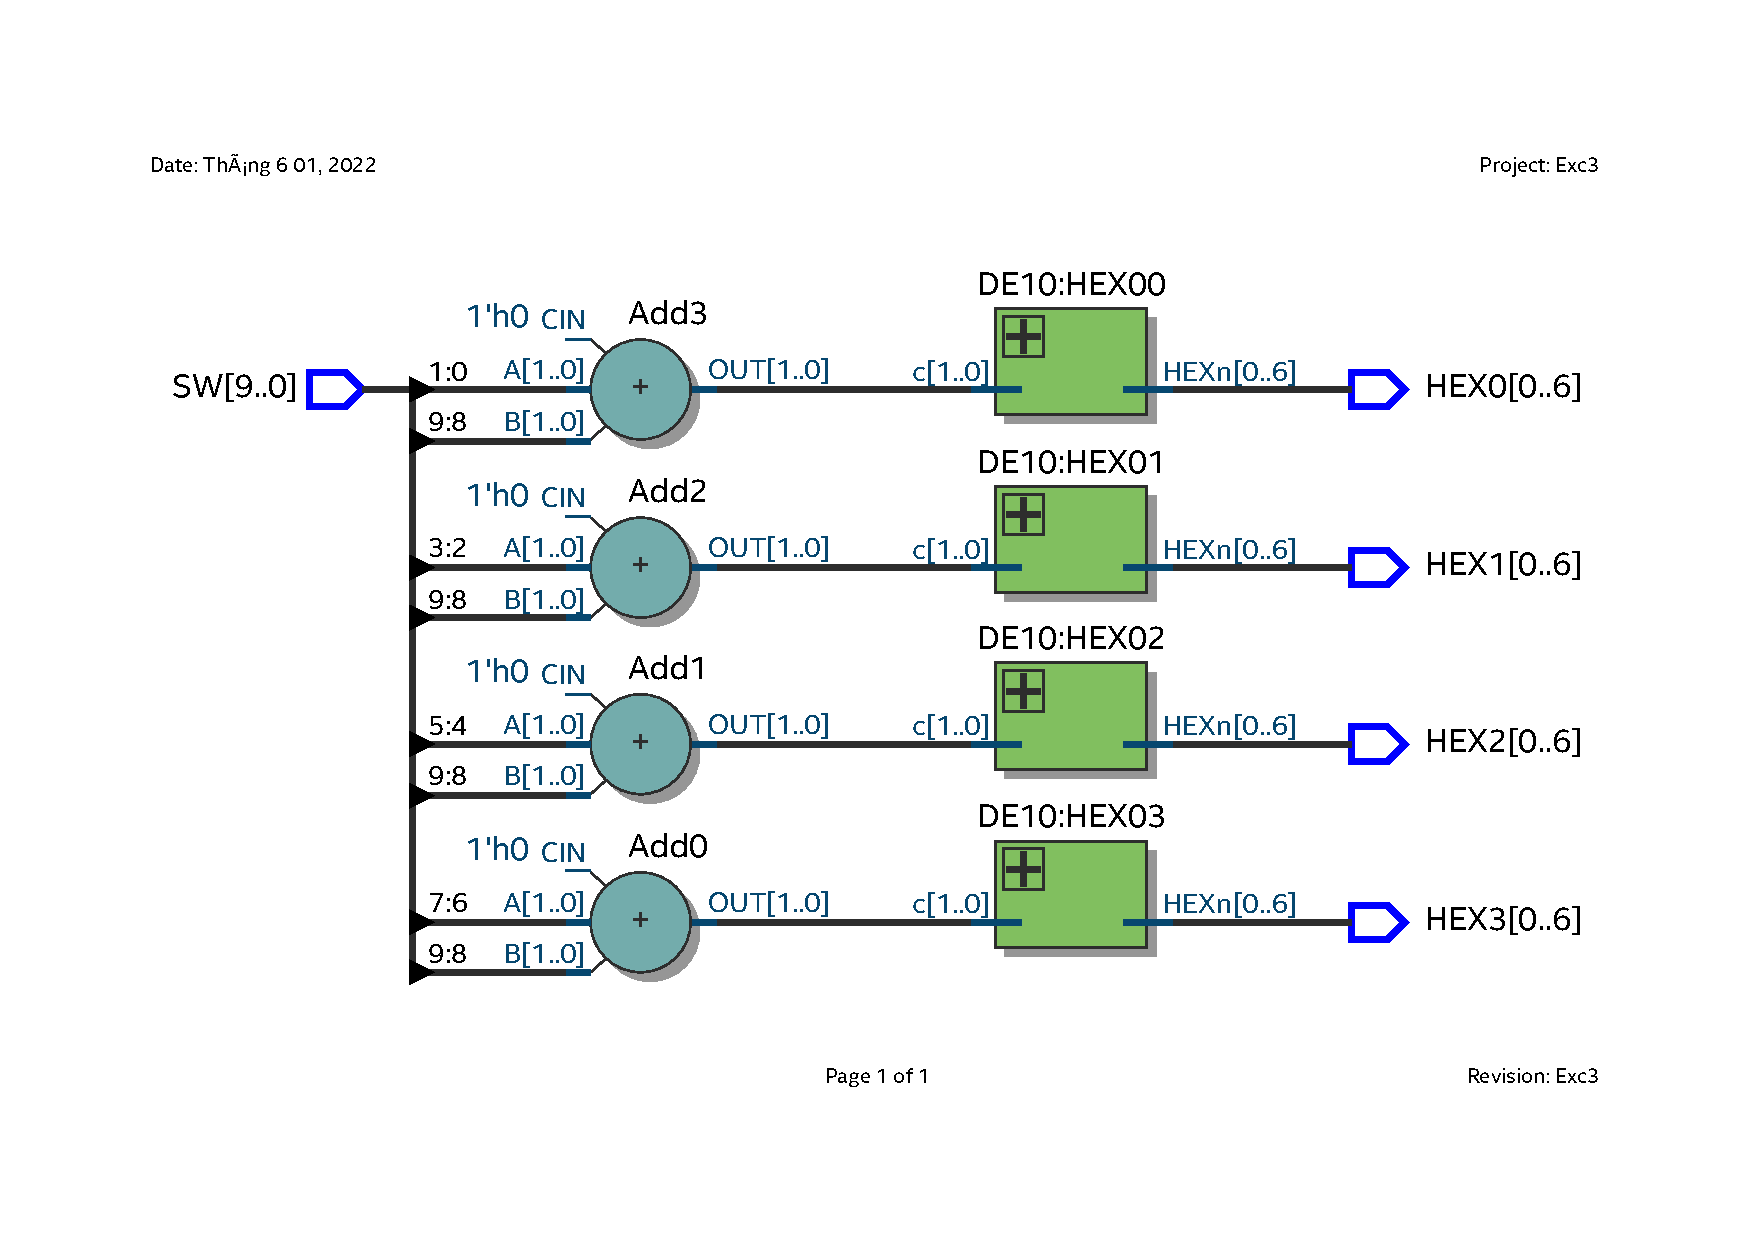
\includegraphics[scale=0.5, clip, trim={2cm 3.8cm 2cm 3.8cm}]{images/Exc3_RTL.pdf}
\caption*{Top level}
\end{figure}

\subsection{Waveform}
\begin{figure}[H]
\centering
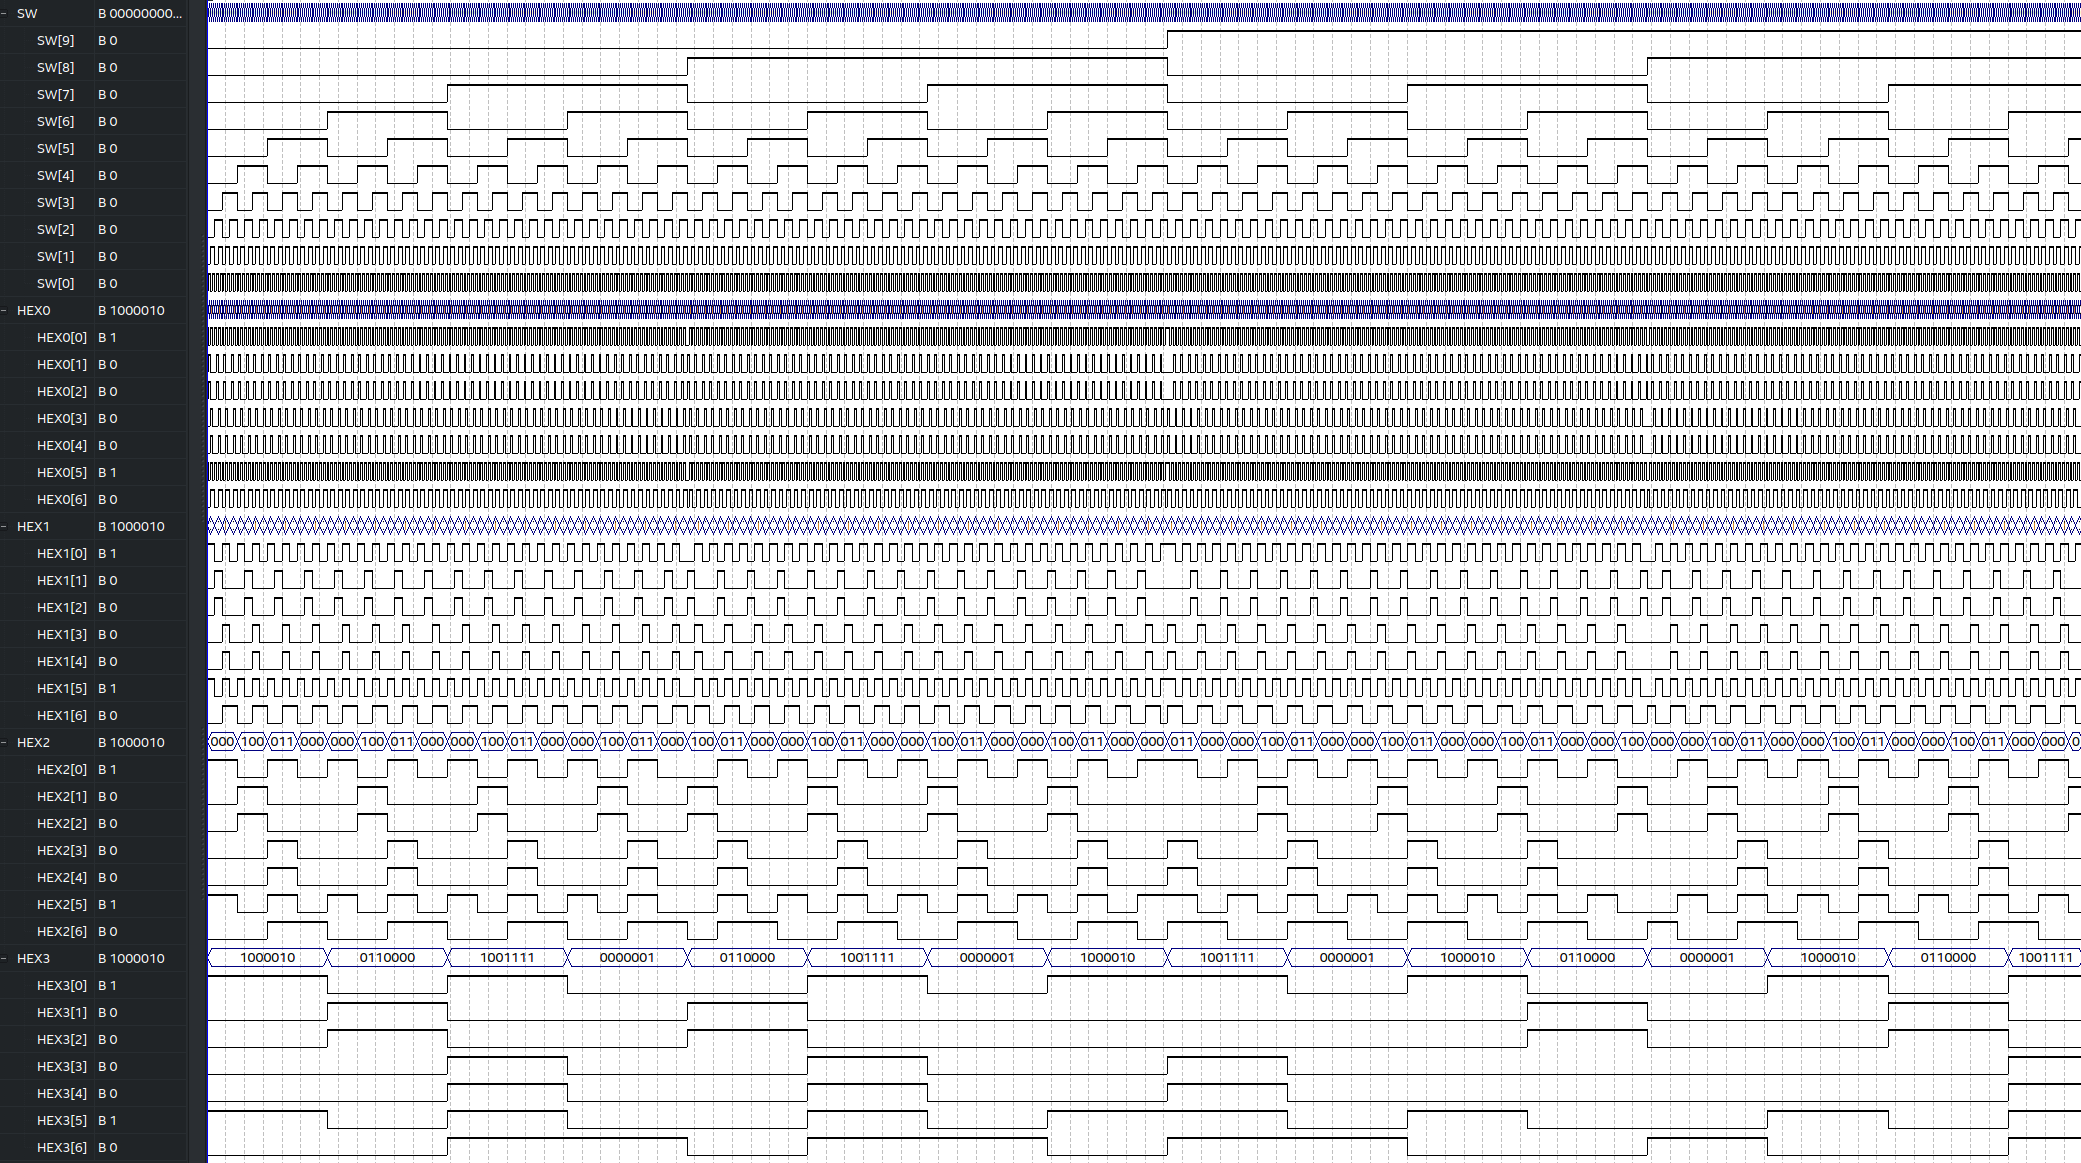
\includegraphics[]{images/Exc3_waveform.png}
\end{figure}

\section{Known how to interface 7-segment LED and multiplexer}

\newcommand{\HELLO}[6]{
\begin{circuitikz}\ctikzset{seven seg/width=0.25, seven seg/thickness=3pt}\draw (#1,0) node[seven segment bits=0110111 dot none box off]{}; \draw (#2,0) node[seven segment val=E dot none box off]{}; \draw (#3,0) node[seven segment bits=0001110 dot none box off]{}; \draw (#4,0) node[seven segment bits=0001110 dot none box off]{}; \draw (#5,0) node[seven segment val=0 dot none box off]{}; \draw (#6,0) node[seven segment val= dot none box off]{};\end{circuitikz}
}

\newcommand{\HELLOb}[6]{
\begin{circuitikz}\ctikzset{seven seg/width=0.25, seven seg/thickness=3pt}\draw (#1,0) node[seven segment val= dot none box off]{}; \draw (#2,0) node[seven segment val= dot none box off]{}; \draw (#3,0) node[seven segment val= dot none box off]{}; \draw (#4,0) node[seven segment val= dot none box off]{}; \draw (#5,0) node[seven segment val= dot none box off]{}; \draw (#6,0) node[seven segment val= dot none box off]{};\end{circuitikz}
}

\begin{table}[H]
\centering
\begin{tabular}{ccc|c}
$s_2$ & $s_1$ & $s_0$ & LEDs                 \\ \hline
0                         & 0     & 0     & \HELLO{0}{1}{2}{3}{4}{5}\\
0                         & 0     & 1     & \HELLO{1}{2}{3}{4}{5}{0}\\
0                         & 1     & 0     & \HELLO{2}{3}{4}{5}{0}{1}\\
0                         & 1     & 1     & \HELLO{3}{4}{5}{0}{1}{2}\\
1                         & 0     & 0     & \HELLO{4}{5}{0}{1}{2}{3}\\
1                         & 0     & 1     & \HELLO{5}{0}{1}{2}{3}{4}\\
1                         & 1     & 0     & \HELLOb{0}{1}{2}{3}{4}{5}\\
1                         & 1     & 1     & \HELLOb{1}{2}{3}{4}{5}{0}
\end{tabular}
\end{table}

\subsection{Code}
\paragraph{HELLO.vhdl}
\begin{minted}{vhdl}
LIBRARY ieee;
USE ieee.std_logic_1164.ALL;

ENTITY HELLO IS
	PORT (
		c : IN std_logic_vector(2 DOWNTO 0);
		HEXn : OUT std_logic_vector(0 TO 6)
	);
END HELLO;

ARCHITECTURE behavior OF HELLO IS
	SIGNAL HEX : std_logic_vector(0 TO 6);
BEGIN
	HEXn <= NOT(HEX);
	WITH c SELECT
	HEX <= "0110111" WHEN "000", 
	       "1001111" WHEN "001", 
	       "0001110" WHEN "010", 
	       "1111110" WHEN "011", 
	       "0000000" WHEN OTHERS;
END behavior;
\end{minted}

\paragraph{Six2OneMUX.vhdl}
\begin{minted}{vhdl}
LIBRARY ieee;
USE ieee.std_logic_1164.ALL;

ENTITY Six2OneMUX IS
	PORT (
		s : IN std_logic_vector(2 DOWNTO 0);
		u : IN std_logic;
		v : IN std_logic;
		w : IN std_logic;
		x : IN std_logic;
		y : IN std_logic;
		z : IN std_logic;
		m : OUT std_logic
	);
END ENTITY;

ARCHITECTURE behave OF Six2OneMUX IS
BEGIN
	WITH s SELECT
	m <= u WHEN "000", 
	     v WHEN "001", 
	     w WHEN "010", 
	     x WHEN "011", 
	     y WHEN "100", 
	     z WHEN "101", 
	     '1' WHEN OTHERS;

END ARCHITECTURE;
\end{minted}

\paragraph{ThreeBitSix2OneMUX.vhdl}
\begin{minted}{vhdl}
LIBRARY ieee;
USE ieee.std_logic_1164.ALL;

ENTITY ThreeBitSix2OneMUX IS
	PORT (
		ss : IN std_logic_vector(2 DOWNTO 0);
		uu : IN std_logic_vector(2 DOWNTO 0);
		vv : IN std_logic_vector(2 DOWNTO 0);
		ww : IN std_logic_vector(2 DOWNTO 0);
		xx : IN std_logic_vector(2 DOWNTO 0);
		yy : IN std_logic_vector(2 DOWNTO 0);
		zz : IN std_logic_vector(2 DOWNTO 0);
		mm : OUT std_logic_vector(2 DOWNTO 0)
	);
END ENTITY;

ARCHITECTURE behave OF ThreeBitSix2OneMUX IS
	COMPONENT Six2OneMUX IS
		PORT (
			s : IN std_logic_vector(2 DOWNTO 0);
			u : IN std_logic;
			v : IN std_logic;
			w : IN std_logic;
			x : IN std_logic;
			y : IN std_logic;
			z : IN std_logic;
			m : OUT std_logic
		);
	END COMPONENT;

BEGIN
	gen : FOR i IN 2 DOWNTO 0 GENERATE
		MUX2 : Six2OneMUX
		PORT MAP(
			s => ss, 
			u => uu(i), 
			v => vv(i), 
			w => ww(i), 
			x => xx(i), 
			y => yy(i), 
			z => zz(i), 
			m => mm(i)
		);
	END GENERATE;

END ARCHITECTURE;
\end{minted}

\paragraph{HELLO.vhdl}
\begin{minted}{vhdl}
LIBRARY ieee;
USE ieee.std_logic_1164.ALL;

ENTITY Exc4 IS
	PORT (
		SW : IN std_logic_vector(2 DOWNTO 0);
		HEX0 : OUT std_logic_vector(0 TO 6);
		HEX1 : OUT std_logic_vector(0 TO 6);
		HEX2 : OUT std_logic_vector(0 TO 6);
		HEX3 : OUT std_logic_vector(0 TO 6);
		HEX4 : OUT std_logic_vector(0 TO 6);
		HEX5 : OUT std_logic_vector(0 TO 6)
	);
END ENTITY;

ARCHITECTURE behave OF Exc4 IS
	SIGNAL sel5, sel4, sel3, sel2, sel1, sel0, selct : std_logic_vector(2 DOWNTO 0);
	SIGNAL outHEX5, outHEX4, outHEX3, outHEX2, outHEX1, outHEX0 : std_logic_vector(2 DOWNTO 0);
 
	COMPONENT HELLO IS
		PORT (
			c : IN std_logic_vector(2 DOWNTO 0);
			HEXn : OUT std_logic_vector(0 TO 6)
		);
	END COMPONENT;
 
	COMPONENT ThreeBitSix2OneMUX IS
		PORT (
			ss : IN std_logic_vector(2 DOWNTO 0);
			uu : IN std_logic_vector(2 DOWNTO 0);
			vv : IN std_logic_vector(2 DOWNTO 0);
			ww : IN std_logic_vector(2 DOWNTO 0);
			xx : IN std_logic_vector(2 DOWNTO 0);
			yy : IN std_logic_vector(2 DOWNTO 0);
			zz : IN std_logic_vector(2 DOWNTO 0);
			mm : OUT std_logic_vector(2 DOWNTO 0)
		);
	END COMPONENT;

BEGIN
	selct <= SW(2 DOWNTO 0);

	-- HELLO
	sel5 <= "000";
	sel4 <= "001";
	sel3 <= "010";
	sel2 <= "010";
	sel1 <= "011";
	sel0 <= "100";

	MUX5 : ThreeBitSix2OneMUX
	PORT MAP(
		uu => sel5, vv => sel0, ww => sel1, xx => sel2, yy => sel3,
		zz => sel4, ss => selct, mm => outHEX5
	);
	MUX4 : ThreeBitSix2OneMUX
	PORT MAP(
		uu => sel4, vv => sel5, ww => sel0, xx => sel1, yy => sel2,
		zz => sel3, ss => selct, mm => outHEX4
	);
	MUX3 : ThreeBitSix2OneMUX
	PORT MAP(
		uu => sel3, vv => sel4, ww => sel5, xx => sel0, yy => sel1,
		zz => sel2, ss => selct, mm => outHEX3
	);
	MUX2 : ThreeBitSix2OneMUX
	PORT MAP(
		uu => sel2, vv => sel3, ww => sel4, xx => sel5, yy => sel0,
		zz => sel1, ss => selct, mm => outHEX2
	);
	MUX1 : ThreeBitSix2OneMUX
	PORT MAP(
		uu => sel1, vv => sel2, ww => sel3, xx => sel4, yy => sel5,
		zz => sel0, ss => selct, mm => outHEX1
	);
	MUX0 : ThreeBitSix2OneMUX
	PORT MAP(
		uu => sel0, vv => sel1, ww => sel2, xx => sel3, yy => sel4,
		zz => sel5, ss => selct, mm => outHEX0
	);
 
	HEX05 : HELLO PORT MAP(c => outHEX5, HEXn => HEX5);
	HEX04 : HELLO PORT MAP(c => outHEX4, HEXn => HEX4);
	HEX03 : HELLO PORT MAP(c => outHEX3, HEXn => HEX3);
	HEX02 : HELLO PORT MAP(c => outHEX2, HEXn => HEX2);
	HEX01 : HELLO PORT MAP(c => outHEX1, HEXn => HEX1);
	HEX00 : HELLO PORT MAP(c => outHEX0, HEXn => HEX0);

END ARCHITECTURE;
\end{minted}

\subsection{Waveform}
\begin{figure}[H]
\centering
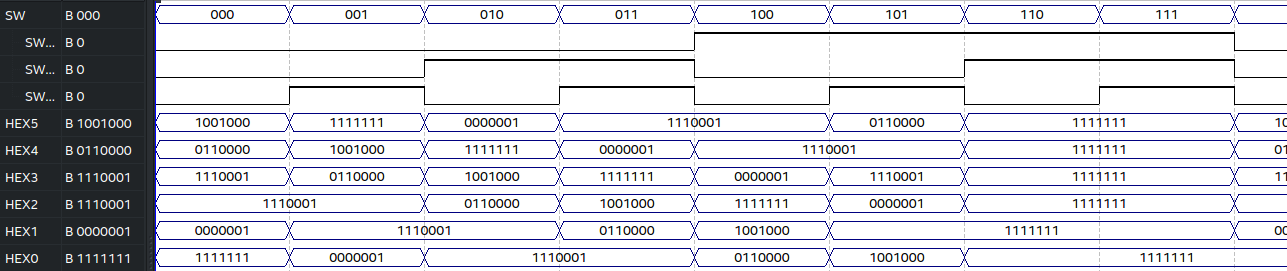
\includegraphics[scale=0.5]{images/Exc4_waveform.png}
\end{figure}

\subsection{Result of RTL viewer}
\begin{figure}[H]
\centering
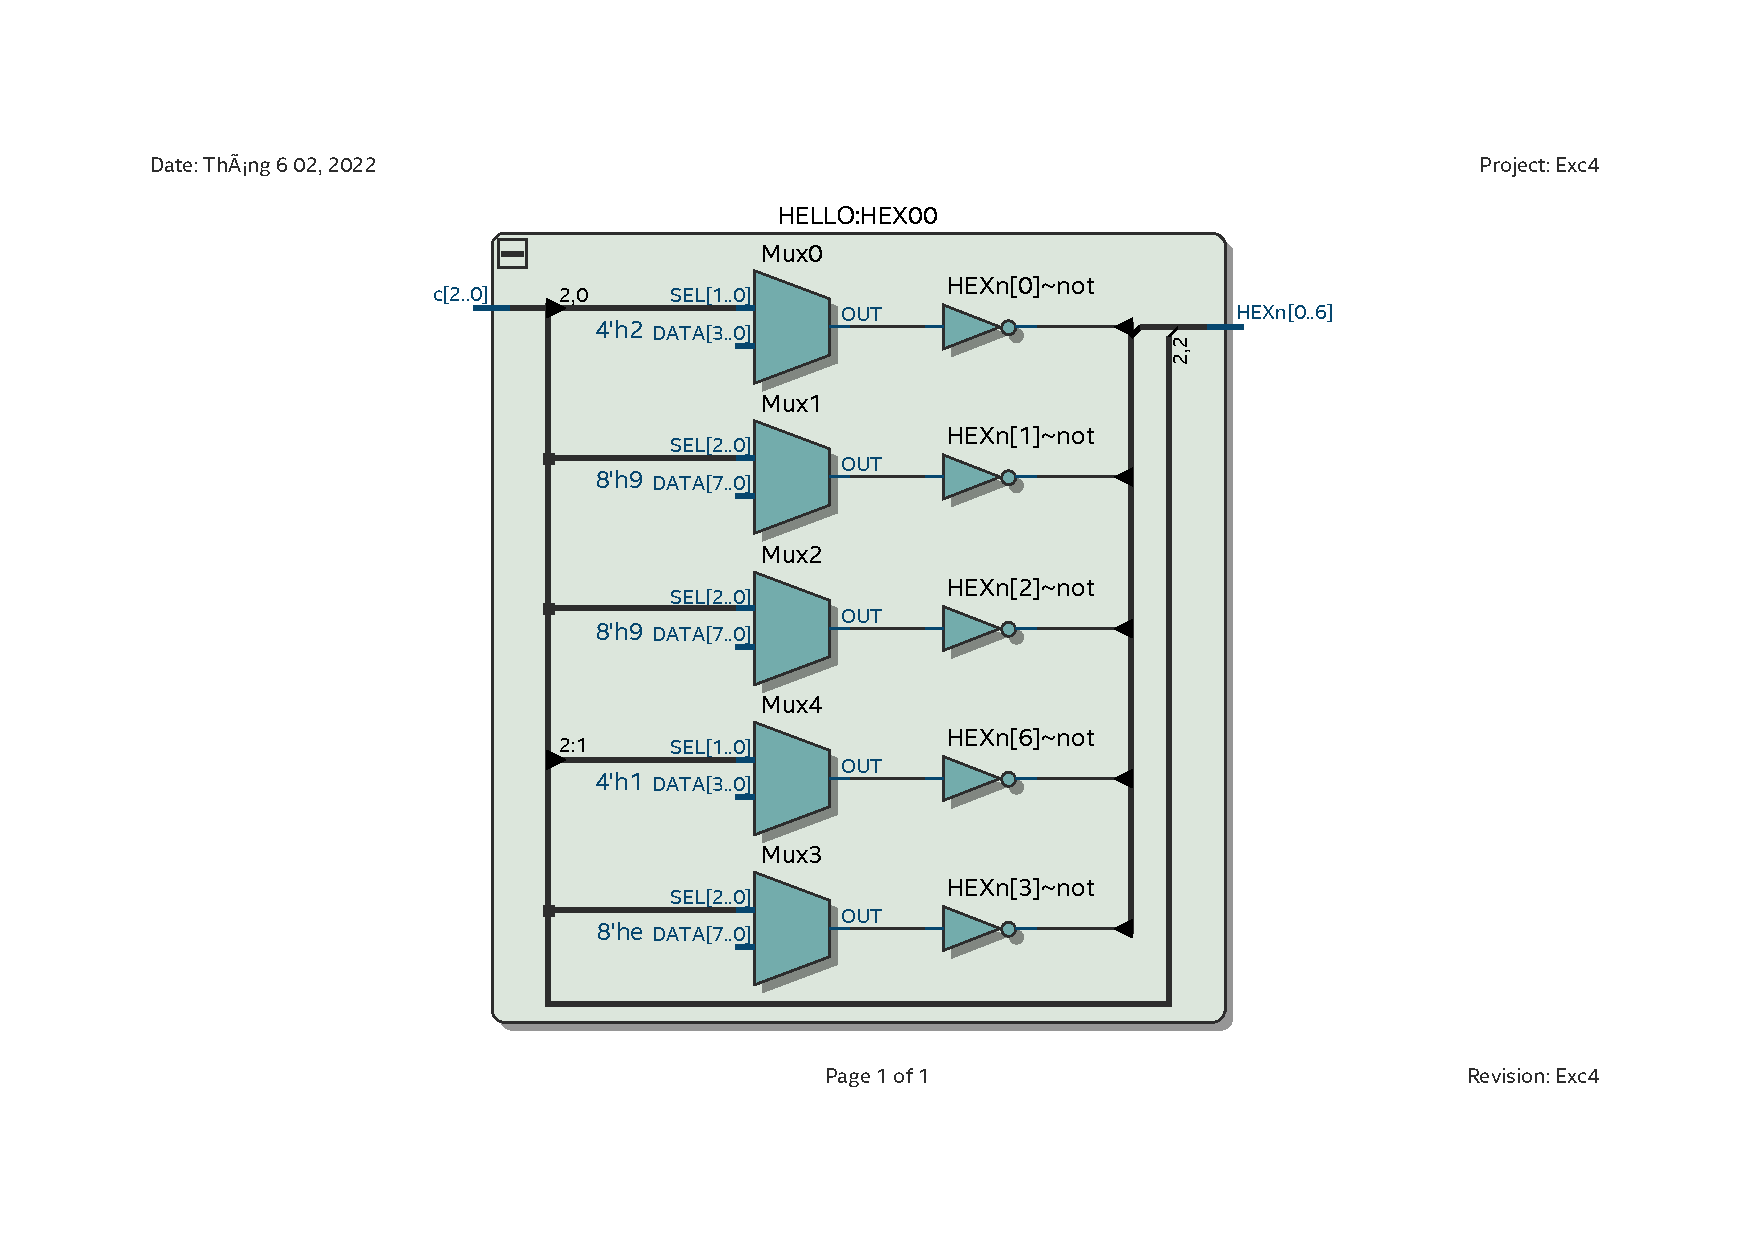
\includegraphics[scale=0.7, clip, trim={2cm 3.5cm 2cm 3.8cm}]{images/Exc4_HELLO_RTL.pdf}
\caption*{``HELLO'' 7-segment decoder}
\end{figure}

\begin{figure}[H]
\centering
\subfloat[][6-to-1 multiplexer]{
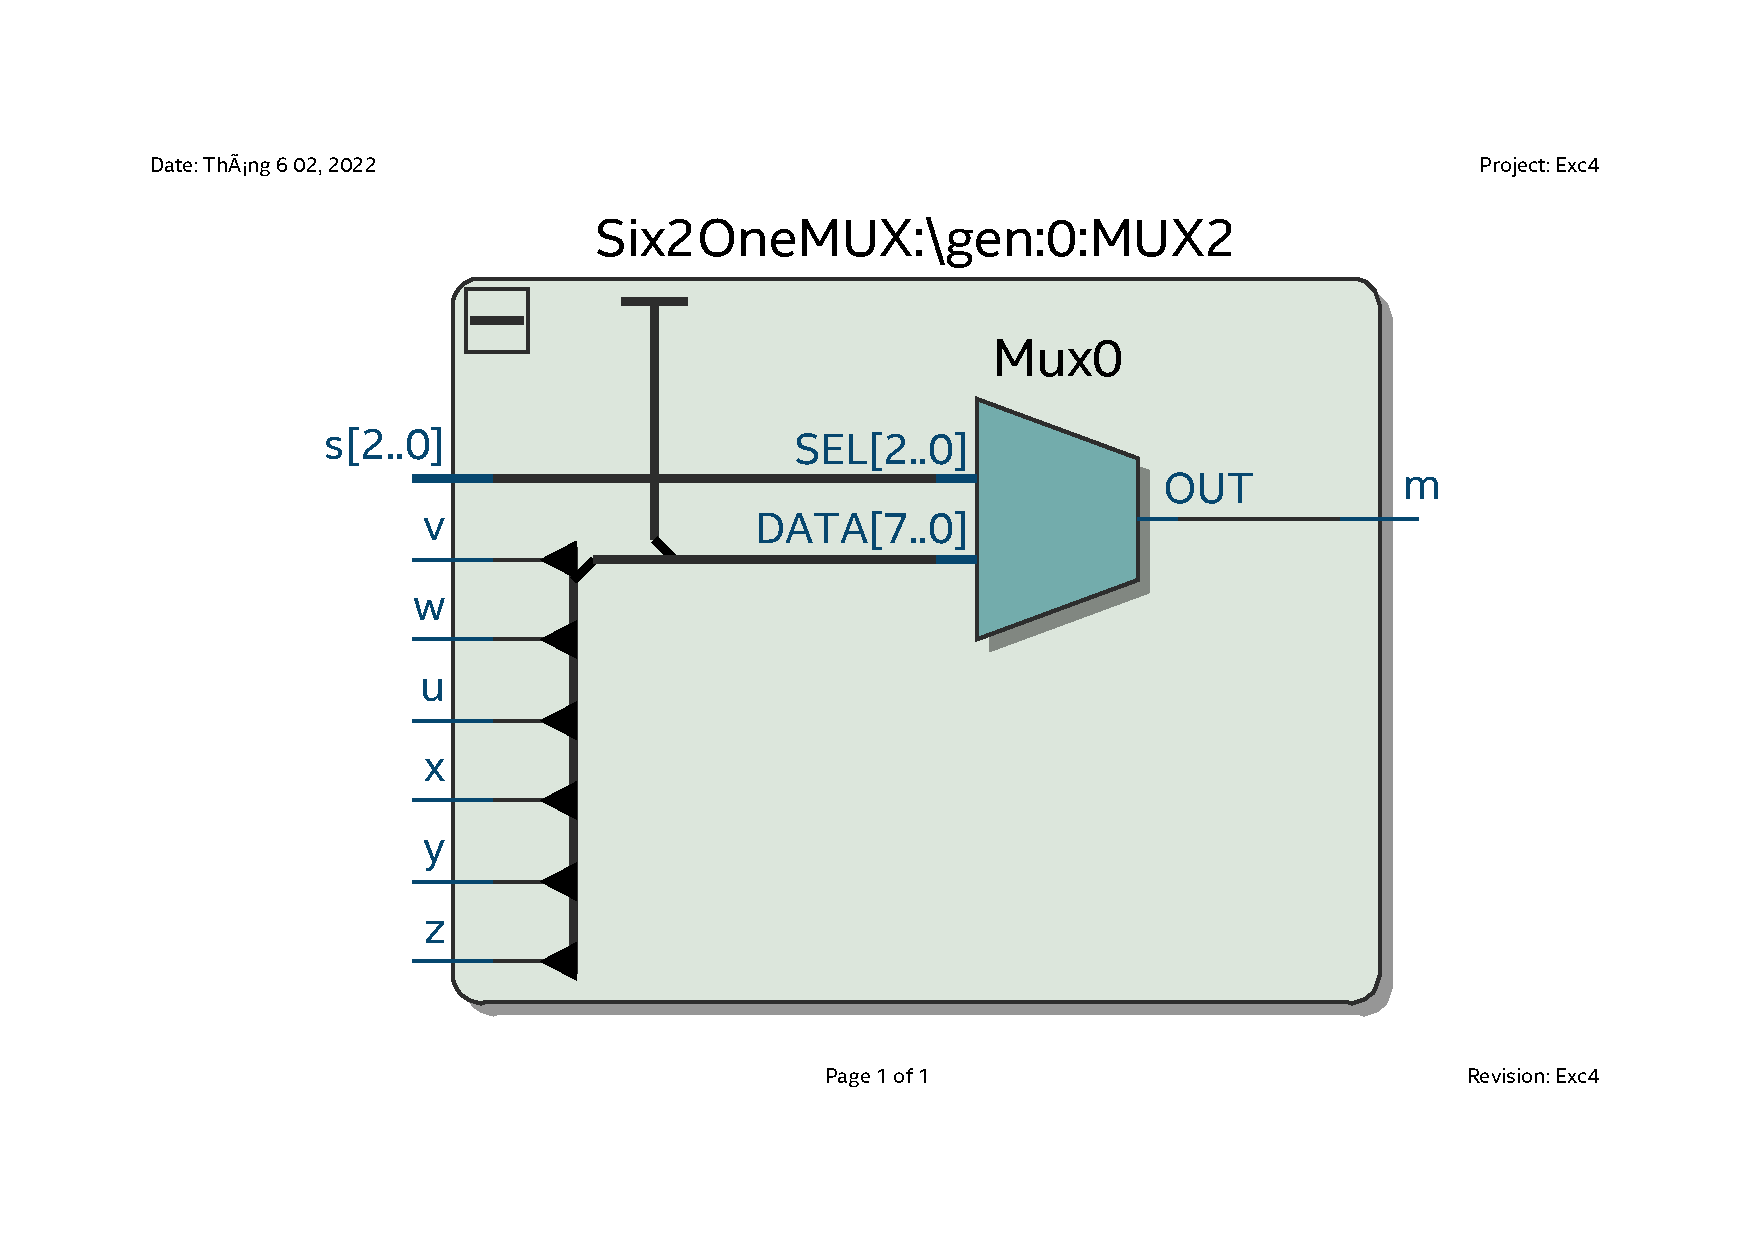
\includegraphics[scale=0.35, clip, trim={3cm 3.5cm 3cm 4.6cm}]{images/Exc4_621MUX_RTL.pdf}}
\subfloat[][3-bit 6-to-1 multiplexer]{
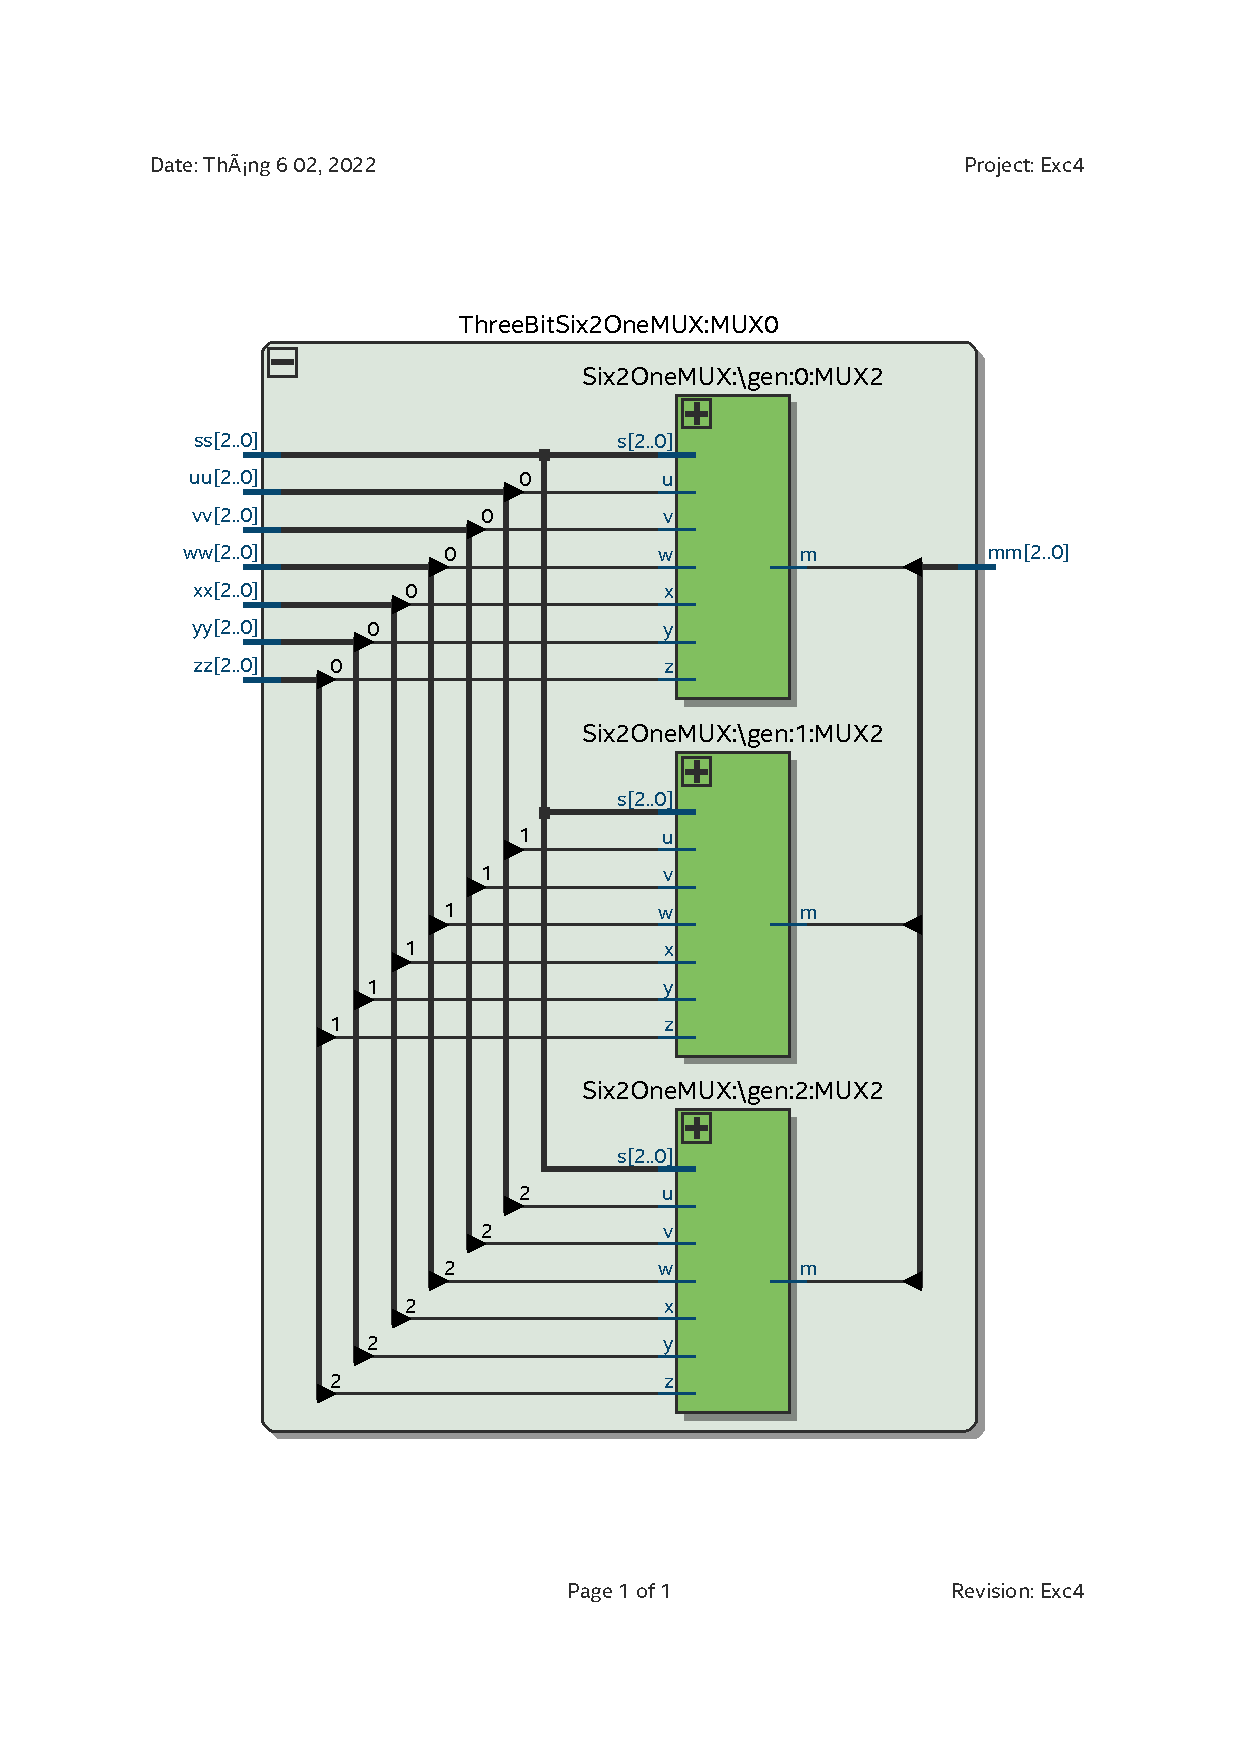
\includegraphics[scale=0.55, clip, trim={3cm 5cm 3cm 5.7cm}]{images/Exc4_3BitMUX_RTL.pdf}}
\end{figure}

\begin{figure}[H]
\centering
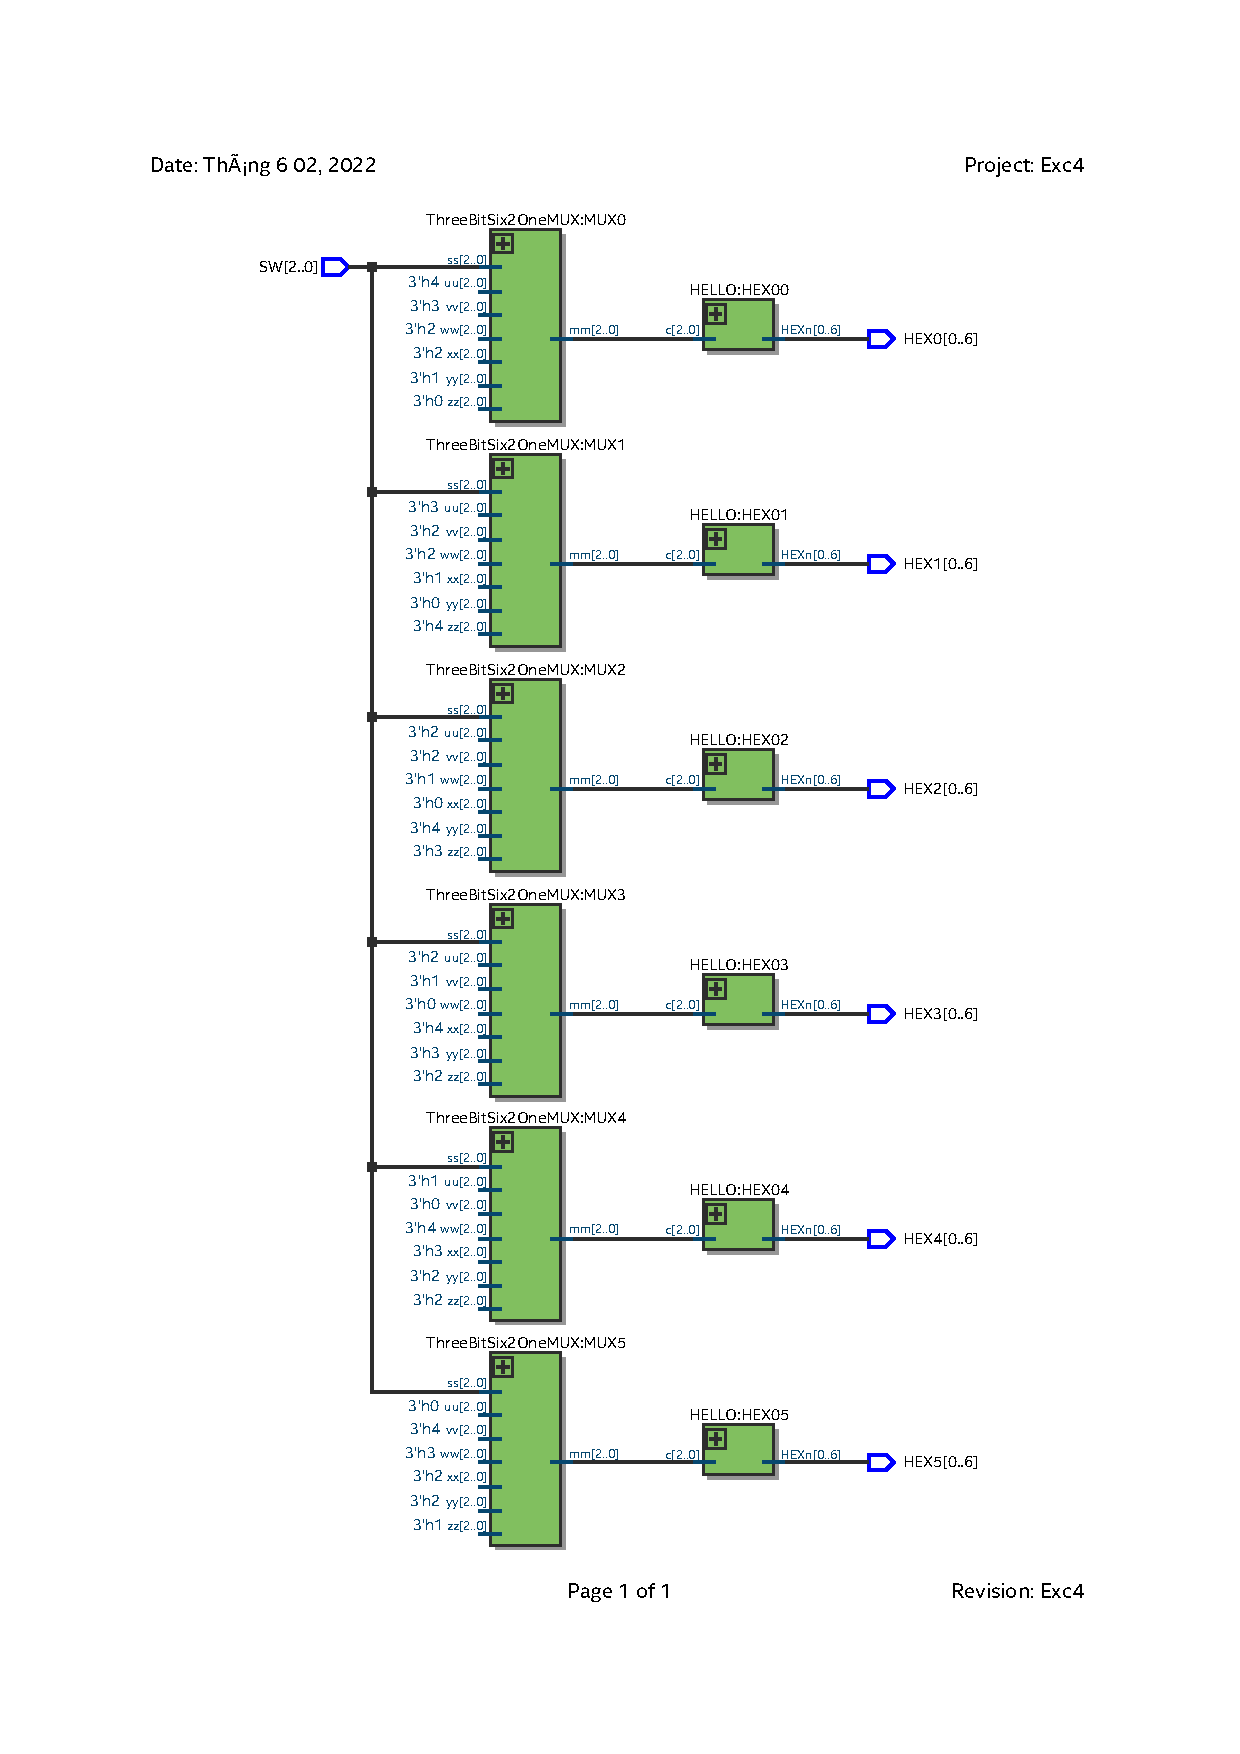
\includegraphics[scale=1, clip, trim={2cm 3.5cm 2cm 3.5cm}]{images/Exc4_RTL.pdf}
\caption*{Top level}
\end{figure}

\section{Known how to interface 7-segment LED and multiplexer}
\newcommand{\BCD}[2]{
\begin{circuitikz}\ctikzset{seven seg/width=0.18, seven seg/thickness=3pt}\draw (0,0) node[seven segment val=#1 dot none box off]{};\draw (1,0) node[seven segment val=#2 dot none box off]{};\end{circuitikz}
}

\begin{table}[H]
\centering
\begin{tabular}{cccc|c}
$v_3$ & $v_2$ & $v_1$ & $v_0$ & $d_1d_0$ \\ \hline
0     & 0     & 0     & 0     & \BCD{0}{0}         \\
0     & 0     & 0     & 1     & \BCD{0}{1}         \\
0     & 0     & 1     & 0     & \BCD{0}{2}         \\
0     & 0     & 1     & 1     & \BCD{0}{3}         \\
0     & 1     & 0     & 0     & \BCD{0}{4}         \\
0     & 1     & 0     & 1     & \BCD{0}{5}         \\
0     & 1     & 1     & 0     & \BCD{0}{6}         \\
0     & 1     & 1     & 1     & \BCD{0}{7}         \\
1     & 0     & 0     & 0     & \BCD{0}{8}         \\
1     & 0     & 0     & 1     & \BCD{0}{9}         \\
1     & 0     & 1     & 0     & \BCD{1}{0}         \\
1     & 0     & 1     & 1     & \BCD{1}{1}         \\
1     & 1     & 0     & 0     & \BCD{1}{2}         \\
1     & 1     & 0     & 1     & \BCD{1}{3}         \\
1     & 1     & 1     & 0     & \BCD{1}{4}         \\
1     & 1     & 1     & 1     & \BCD{1}{5}        
\end{tabular}
\end{table}

\subsection{Method 1: with MUX, comparator and ``Circuit A''}
\subsubsection{Truth tables and functions}

\begin{minipage}[t]{0.5\textwidth}
{\bf \normalsize Comparator $>9$}
\begin{table}[H]
\centering
\begin{tabular}{cccc|c}
$v_3$ & $v_2$ & $v_1$ & $v_0$ & $z$ \\ \hline
0     & 0     & 0     & 0     & 0   \\
0     & 0     & 0     & 1     & 0   \\
0     & 0     & 1     & 0     & 0   \\
0     & 0     & 1     & 1     & 0   \\
0     & 1     & 0     & 0     & 0   \\
0     & 1     & 0     & 1     & 0   \\
0     & 1     & 1     & 0     & 0   \\
0     & 1     & 1     & 1     & 0   \\
1     & 0     & 0     & 0     & 0   \\
1     & 0     & 0     & 1     & 0   \\
1     & 0     & 1     & 0     & 1   \\
1     & 0     & 1     & 1     & 1   \\
1     & 1     & 0     & 0     & 1   \\
1     & 1     & 0     & 1     & 1   \\
1     & 1     & 1     & 0     & 1   \\
1     & 1     & 1     & 1     & 1  
\end{tabular}

$\Rightarrow z=v_3(v_2+v_1)$
\end{table}
\end{minipage}
\begin{minipage}[t]{0.5\textwidth}
{\bf \normalsize Circuit A}
\begin{table}[H]
\centering
\begin{tabular}{cccc|cccc}
$v_3$ & $v_2$ & $v_1$ & $v_0$ & $A_3$    & $A_2$    & $A_1$    & $A_0$    \\ \hline
0     & 0     & 0     & 0     & $\times$ & $\times$ & $\times$ & $\times$ \\
0     & 0     & 0     & 1     & $\times$ & $\times$ & $\times$ & $\times$ \\
0     & 0     & 1     & 0     & $\times$ & $\times$ & $\times$ & $\times$ \\
0     & 0     & 1     & 1     & $\times$ & $\times$ & $\times$ & $\times$ \\
0     & 1     & 0     & 0     & $\times$ & $\times$ & $\times$ & $\times$ \\
0     & 1     & 0     & 1     & $\times$ & $\times$ & $\times$ & $\times$ \\
0     & 1     & 1     & 0     & $\times$ & $\times$ & $\times$ & $\times$ \\
0     & 1     & 1     & 1     & $\times$ & $\times$ & $\times$ & $\times$ \\
1     & 0     & 0     & 0     & $\times$ & $\times$ & $\times$ & $\times$ \\
1     & 0     & 0     & 1     & $\times$ & $\times$ & $\times$ & $\times$ \\
1     & 0     & 1     & 0     & 0        & 0        & 0        & 0        \\
1     & 0     & 1     & 1     & 0        & 0        & 0        & 1        \\
1     & 1     & 0     & 0     & 0        & 0        & 1        & 0        \\
1     & 1     & 0     & 1     & 0        & 0        & 1        & 1        \\
1     & 1     & 1     & 0     & 0        & 1        & 0        & 0        \\
1     & 1     & 1     & 1     & 0        & 1        & 0        & 1       
\end{tabular}

$\Rightarrow \begin{array}{rcl}
A_3 & = & 0 \\
A_2 & = & v_2v_1 \\
A_1 & = & \bar v_1\\
A_0 & = & v_0
\end{array}$
\end{table}
\end{minipage}


\subsubsection{Code}
\paragraph{BCD.vhdl}
\begin{minted}{vhdl}
LIBRARY ieee;
USE ieee.std_logic_1164.ALL;

ENTITY BCD IS
	PORT (
		c : IN std_logic_vector(3 DOWNTO 0);
		HEXn : OUT std_logic_vector(0 TO 6)
	);
END BCD;

ARCHITECTURE behavior OF BCD IS
	SIGNAL HEX : std_logic_vector(0 TO 6);
BEGIN
	HEXn <= NOT(HEX);
	WITH c SELECT
	HEX <= "1111110" WHEN "0000", 
	       "0110000" WHEN "0001", 
	       "1101101" WHEN "0010", 
	       "1111001" WHEN "0011", 
	       "0110011" WHEN "0100", 
	       "1011011" WHEN "0101", 
	       "1011111" WHEN "0110", 
	       "1110000" WHEN "0111", 
	       "1111111" WHEN "1000", 
	       "1111011" WHEN "1001", 
	       "0000000" WHEN OTHERS;
END behavior;
\end{minted}

\paragraph{MUX.vhdl}
\begin{minted}{vhdl}
LIBRARY ieee;
USE ieee.std_logic_1164.ALL;

ENTITY MUX IS
	PORT (
		muxIn1 : IN std_logic;
		muxSel : IN std_logic;
		muxIn2 : IN std_logic;
		muxOut : OUT std_logic
	);
END ENTITY;

ARCHITECTURE arch OF MUX IS
BEGIN
	muxOut <= (NOT(muxSel) AND muxIn1) OR (muxSel AND muxIn2);
END arch;
\end{minted}

\paragraph{FourBitMUX.vhdl}
\begin{minted}{vhdl}
LIBRARY ieee;
USE ieee.std_logic_1164.ALL;

ENTITY FourBitMUX IS
	PORT (
		fourBitMuxIn1 : IN std_logic_vector(3 DOWNTO 0);
		fourBitMuxIn2 : IN std_logic_vector(3 DOWNTO 0);
		fourBitMuxSel : IN std_logic;
		fourBitMuxOut : OUT std_logic_vector(3 DOWNTO 0)
	);
END ENTITY;

ARCHITECTURE arch OF FourBitMUX IS
	COMPONENT MUX
		PORT (
			muxIn1 : IN std_logic;
			muxSel : IN std_logic;
			muxIn2 : IN std_logic;
			muxOut : OUT std_logic
		);
	END COMPONENT;
BEGIN
	gen : FOR i IN 3 DOWNTO 0 GENERATE
		MUX2 : MUX
		PORT MAP(
			muxSel => fourBitMuxSel, 
			muxIn1 => fourBitMuxIn1(i), 
			muxIn2 => fourBitMuxIn2(i), 
			muxOut => fourBitMuxOut(i)
		);
	END GENERATE;
END arch;
\end{minted}

\paragraph{Comparator.vhdl}
\begin{minted}{vhdl}
LIBRARY ieee;
USE ieee.std_logic_1164.ALL;

ENTITY Comparator IS
	PORT (
		compIn : IN std_logic_vector(3 DOWNTO 0);
		compOut : OUT std_logic
	);
END ENTITY;

ARCHITECTURE behave OF Comparator IS
BEGIN
	-- Z = A(B+C)
	compOut <= compIn(3) AND (compIn(2) OR compIn(1));

END ARCHITECTURE;
\end{minted}

\paragraph{CircuitA.vhdl}
\begin{minted}{vhdl}
LIBRARY ieee;
USE ieee.std_logic_1164.ALL;

ENTITY CircuitA IS
	PORT (
		dIn : IN std_logic_vector(3 DOWNTO 0);
		dOut : OUT std_logic_vector(3 DOWNTO 0)
	);
END ENTITY;

ARCHITECTURE behave OF CircuitA IS
BEGIN
	dOut(3) <= '0';
	dOut(2) <= dIn(2) AND dIn(1);
	dOut(1) <= NOT(dIn(1));
	dOut(0) <= dIn(0);

END ARCHITECTURE;
\end{minted}

\paragraph{Exc5.vhdl}
\begin{minted}{vhdl}
LIBRARY ieee;
USE ieee.std_logic_1164.ALL;

ENTITY Exc5 IS
	PORT (
		V : IN std_logic_vector(3 DOWNTO 0);
		HEX0 : OUT std_logic_vector(0 TO 6);
		HEX1 : OUT std_logic_vector(0 TO 6)
	);
END ENTITY;

ARCHITECTURE behave OF Exc5 IS

	SIGNAL z : std_logic;
	SIGNAL A, m : std_logic_vector(3 DOWNTO 0);

	COMPONENT FourBitMUX IS
		PORT (
			fourBitMuxIn1 : IN std_logic_vector(3 DOWNTO 0);
			fourBitMuxIn2 : IN std_logic_vector(3 DOWNTO 0);
			fourBitMuxSel : IN std_logic;
			fourBitMuxOut : OUT std_logic_vector(3 DOWNTO 0)
		);
	END COMPONENT;
 
	COMPONENT Comparator IS
		PORT (
			compIn : IN std_logic_vector(3 DOWNTO 0);
			compOut : OUT std_logic
		);
	END COMPONENT;

	COMPONENT CircuitA IS
		PORT (
			dIn : IN std_logic_vector(3 DOWNTO 0);
			dOut : OUT std_logic_vector(3 DOWNTO 0)
		);
	END COMPONENT;

	COMPONENT BCD IS
		PORT (
			c : IN std_logic_vector(3 DOWNTO 0);
			HEXn : OUT std_logic_vector(0 TO 6)
		);
	END COMPONENT;
 
BEGIN
	comp : Comparator PORT MAP( compIn => V, compOut => z);
	cirA : CircuitA PORT MAP(dIn => V, dOut => A);
	mux : FourBitMUX
	PORT MAP(
		fourBitMuxIn1 => V, 
		fourBitMuxIn2 => A, 
		fourBitMuxSel => z, 
		fourBitMuxOut => m
	);

	HEX01 : BCD PORT MAP(c => "000" & z, HEXn => HEX1);
	HEX00 : BCD PORT MAP(c => m, HEXn => HEX0);

END ARCHITECTURE;
\end{minted}

\subsubsection{Result of RTL viewer}
\begin{figure}[H]
\centering
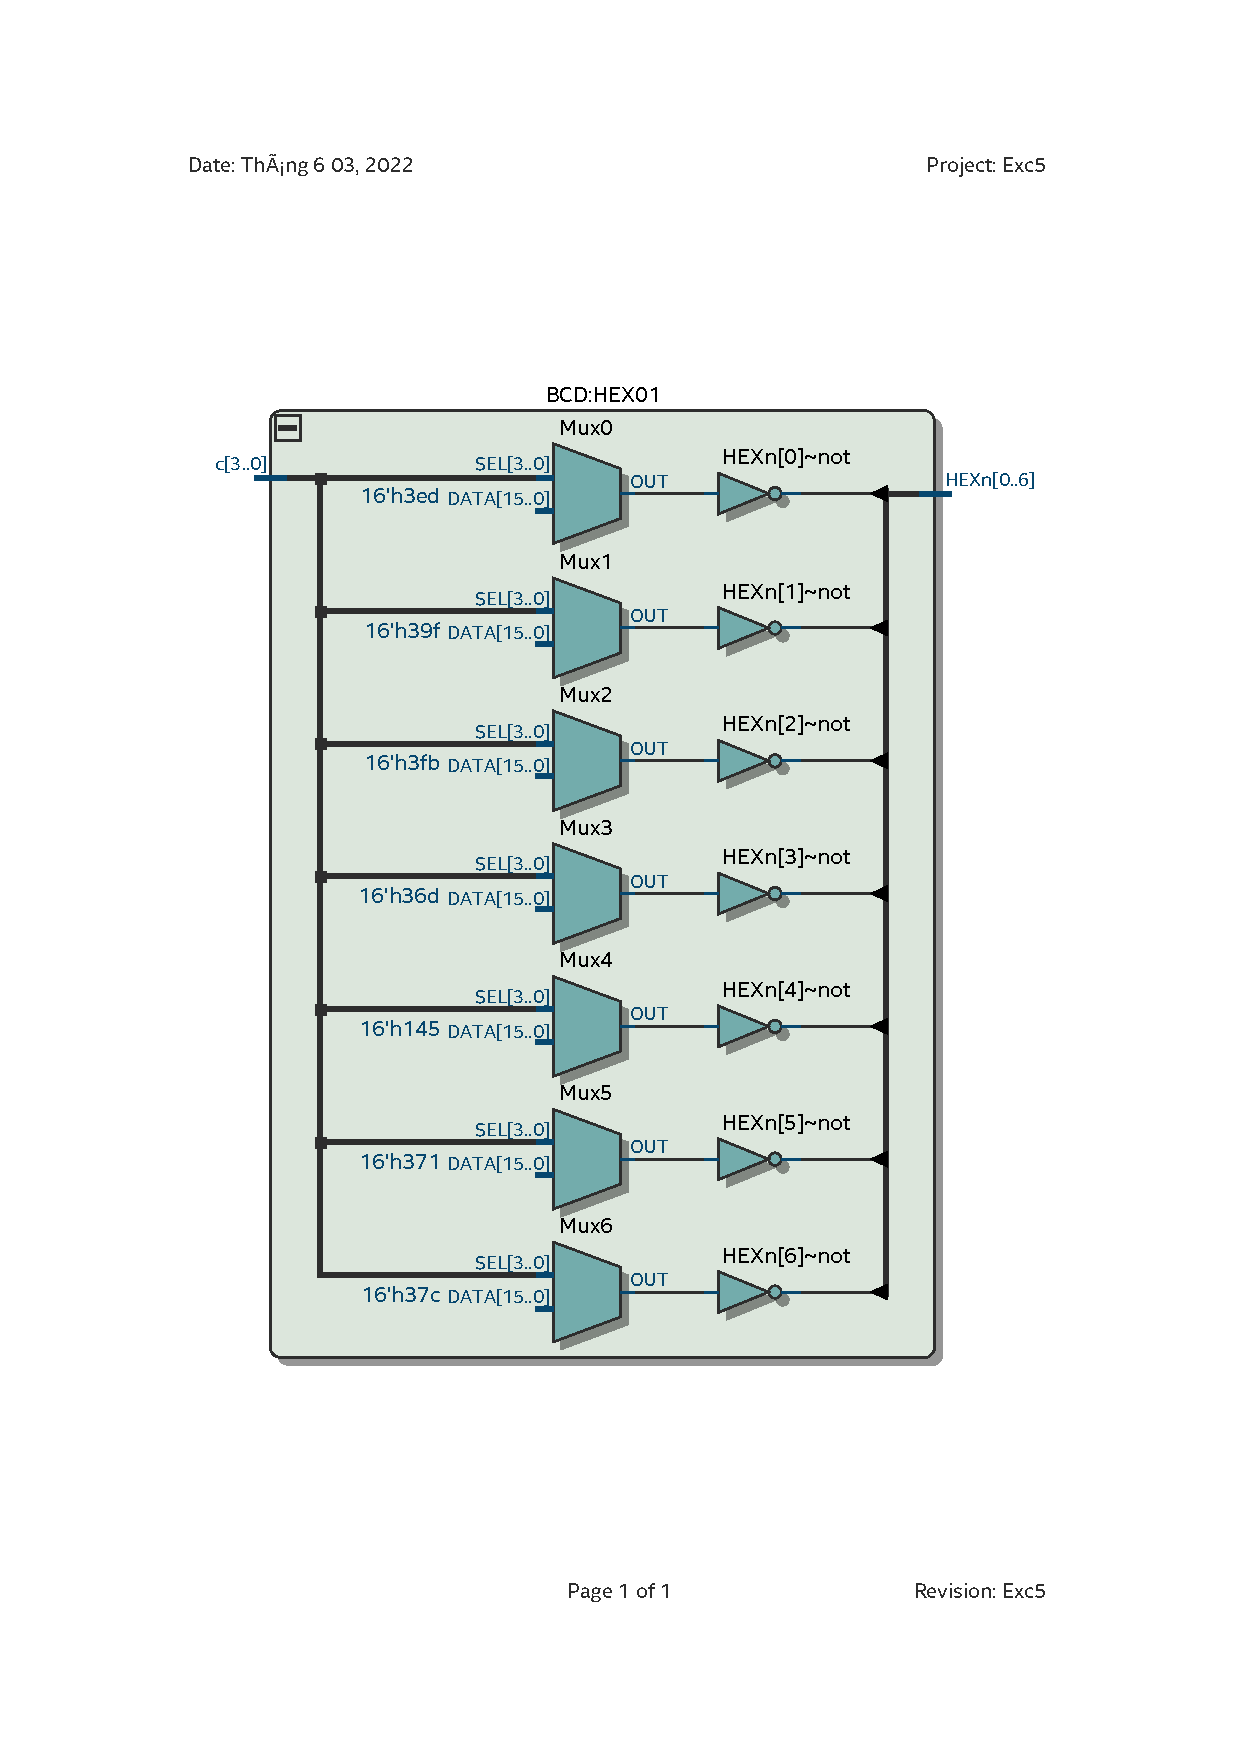
\includegraphics[scale=0.7, clip, trim={2cm 6.6cm 2cm 6.9cm}]{images/Exc5_BCD_RTL.pdf}
\caption*{BCD 7-segment decoder}
\end{figure}

\begin{figure}[H]
\centering
\subfloat[][2-to-1 multiplexer]{
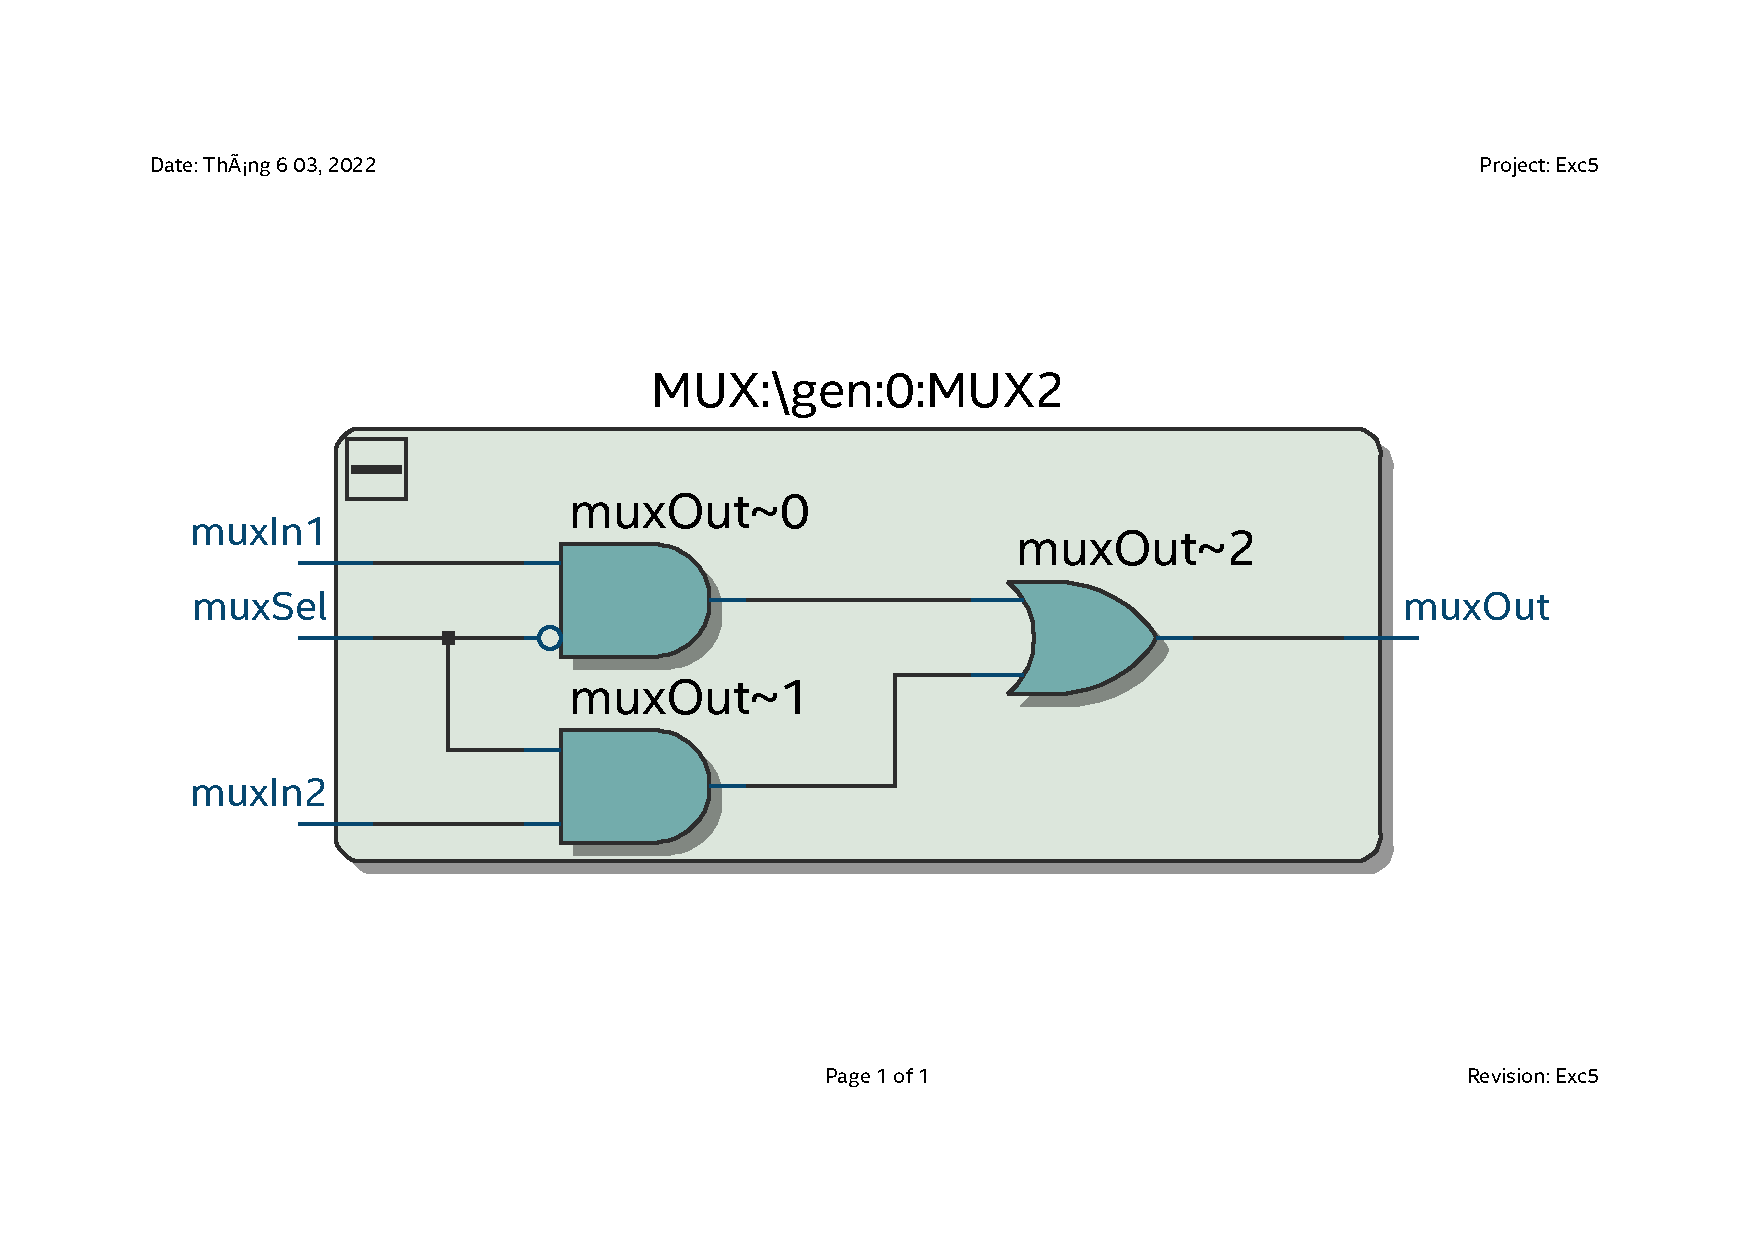
\includegraphics[scale=0.35, clip, trim={3cm 4.8cm 3cm 7.2cm}]{images/Exc5_MUX_RTL.pdf}}
\subfloat[][4-bit 2-to-1 multiplexer]{
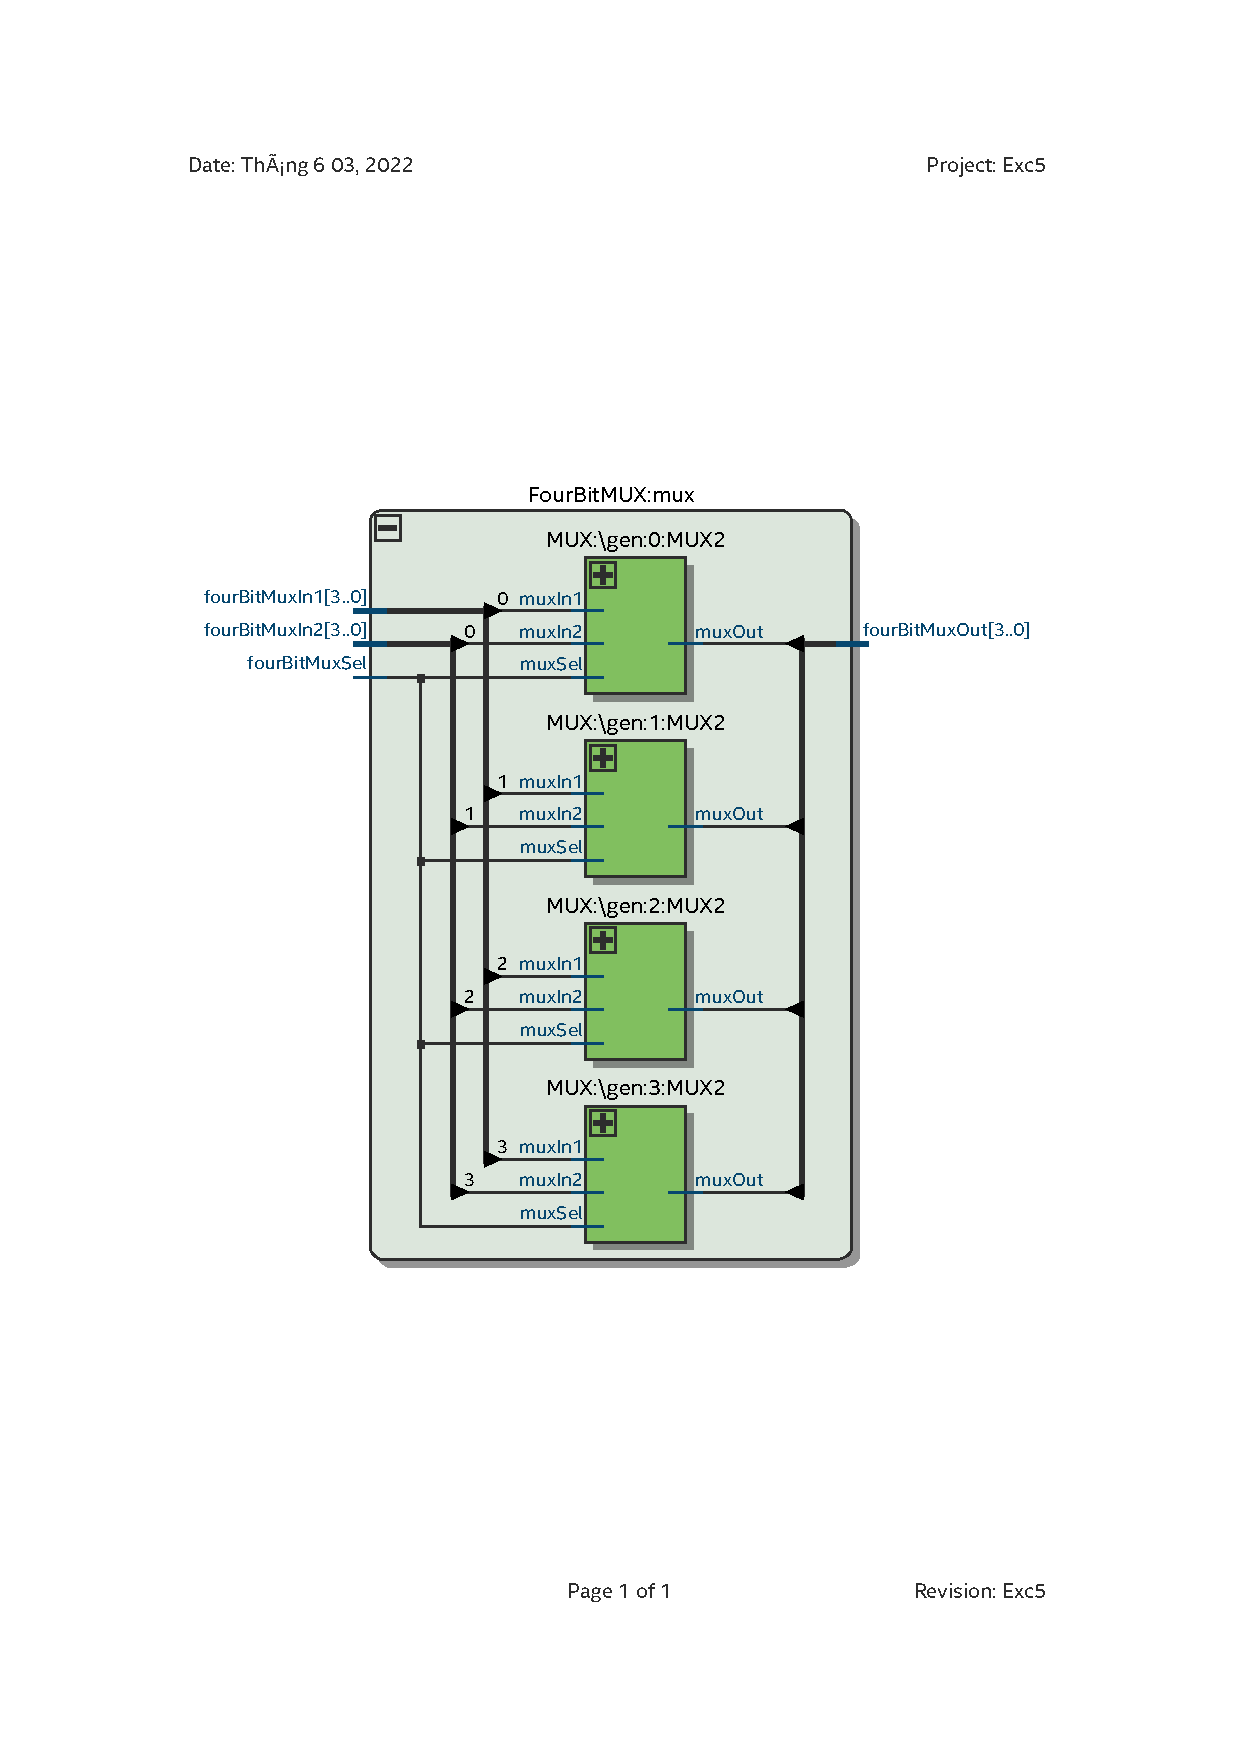
\includegraphics[scale=0.64, clip, trim={3cm 7.5cm 3cm 8.6cm}]{images/Exc5_FourBitMUX_RTL.pdf}}
\end{figure}

\begin{figure}[H]
\centering
\subfloat[][Comparator $>9$]{
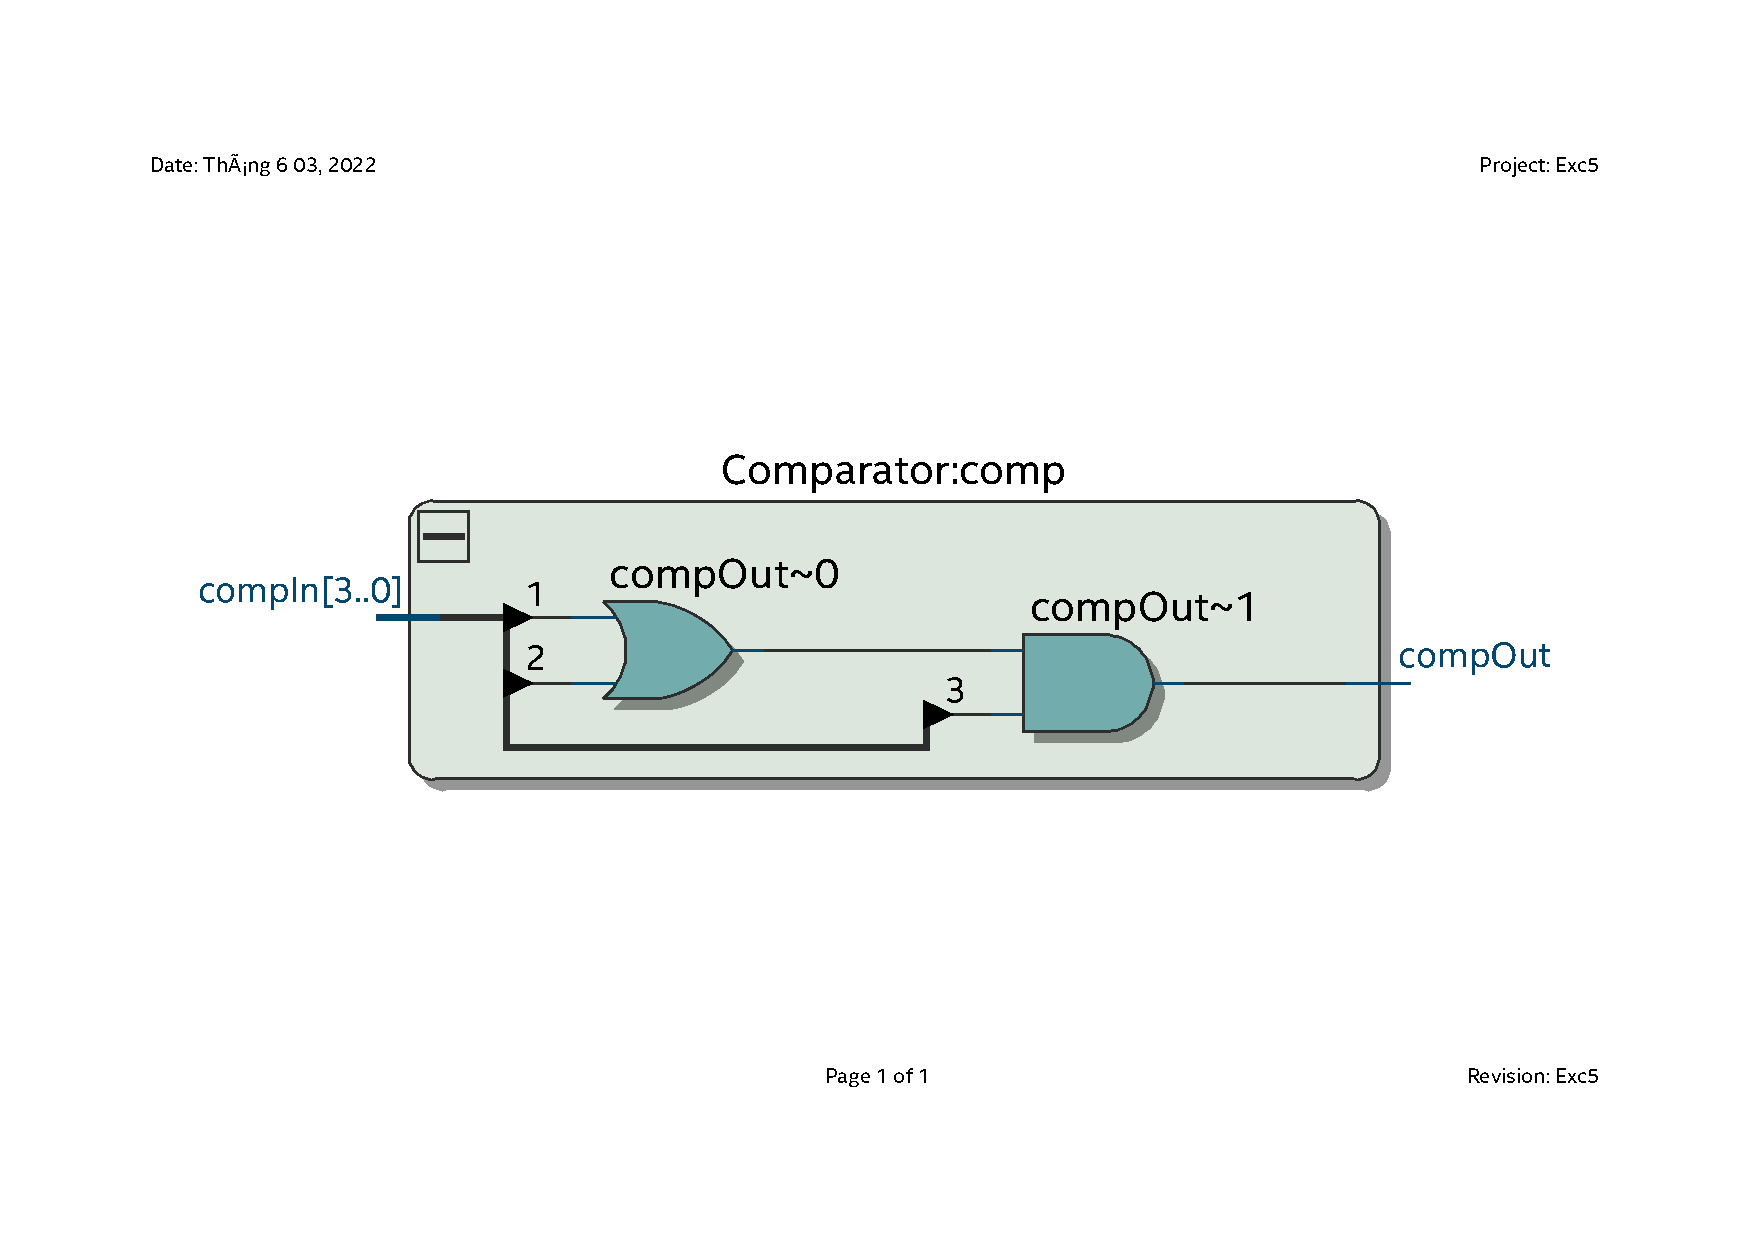
\includegraphics[scale=0.35, clip, trim={3cm 7cm 3cm 8.5cm}]{images/Exc5_Comparator_RTL.pdf}}
\subfloat[][Circuit A]{
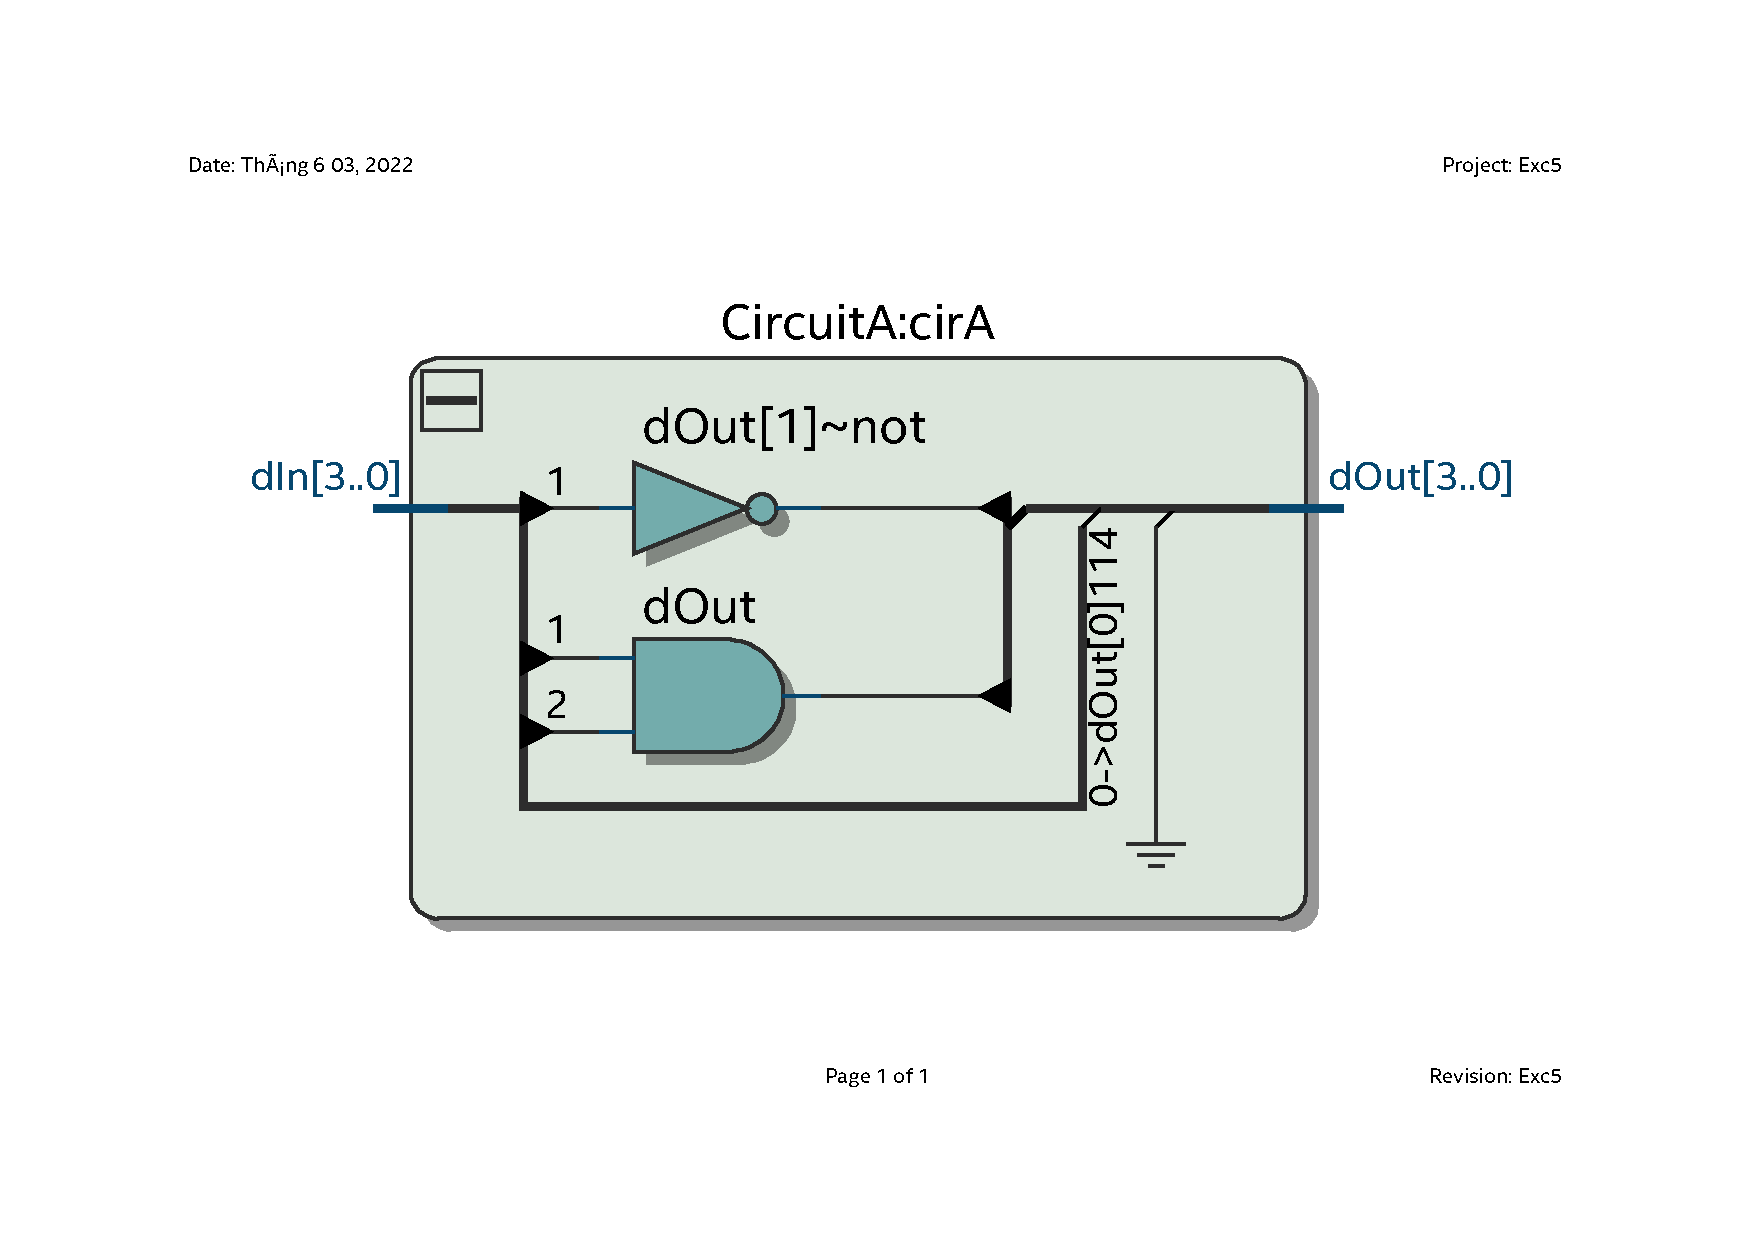
\includegraphics[scale=0.35, clip, trim={3cm 5cm 3cm 6cm}]{images/Exc5_CircuitA_RTL.pdf}}
\end{figure}

\begin{figure}[H]
\centering
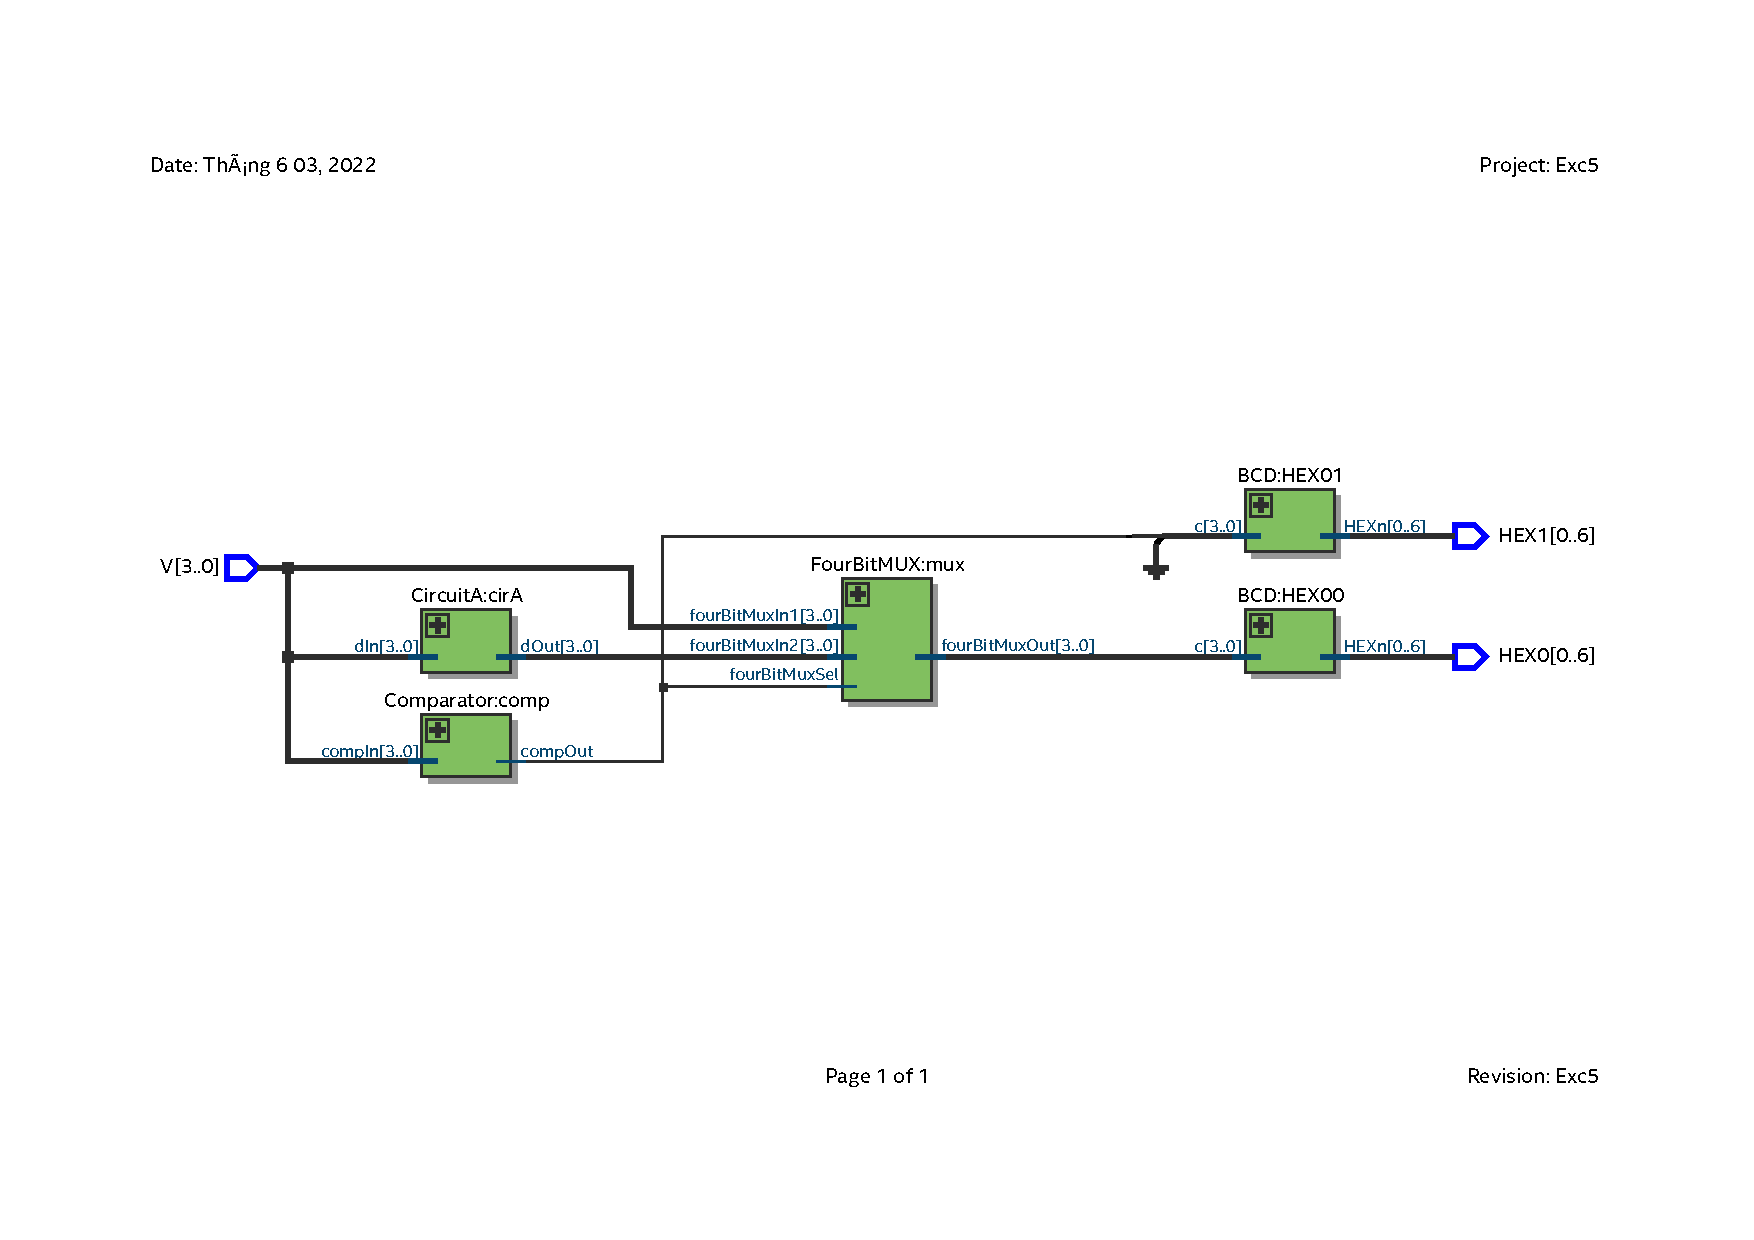
\includegraphics[scale=0.7, clip, trim={2cm 7cm 2cm 7cm}]{images/Exc5_RTL.pdf}
\caption*{Top level}
\end{figure}

\subsection{Method 2: using conditions in VHDL}
\paragraph{BCD.vhdl}
\begin{minted}{vhdl}
LIBRARY ieee;
USE ieee.std_logic_1164.ALL;

ENTITY BCD IS
	PORT (
		c : IN std_logic_vector(3 DOWNTO 0);
		HEXn : OUT std_logic_vector(0 TO 6)
	);
END BCD;

ARCHITECTURE behavior OF BCD IS
	SIGNAL HEX : std_logic_vector(0 TO 6);
BEGIN
	HEXn <= NOT(HEX);
	WITH c SELECT
	HEX <= "1111110" WHEN "0000", 
	       "0110000" WHEN "0001", 
	       "1101101" WHEN "0010", 
	       "1111001" WHEN "0011", 
	       "0110011" WHEN "0100", 
	       "1011011" WHEN "0101", 
	       "1011111" WHEN "0110", 
	       "1110000" WHEN "0111", 
	       "1111111" WHEN "1000", 
	       "1111011" WHEN "1001", 
	       "0000000" WHEN OTHERS;
END behavior;
\end{minted}

\paragraph{Exc5.vhdl}
\begin{minted}{vhdl}
LIBRARY ieee;
USE ieee.std_logic_1164.ALL;
USE IEEE.numeric_std.ALL;

ENTITY Exc5 IS
	PORT (
		V : IN std_logic_vector(3 DOWNTO 0);
		HEX0 : OUT std_logic_vector(0 TO 6);
		HEX1 : OUT std_logic_vector(0 TO 6)
	);
END ENTITY;

ARCHITECTURE behave OF Exc5 IS

	SIGNAL digit1, digit0 : std_logic_vector(3 DOWNTO 0);
 
	COMPONENT BCD IS
		PORT (
			c : IN std_logic_vector(3 DOWNTO 0);
			HEXn : OUT std_logic_vector(0 TO 6)
		);
	END COMPONENT;
 

BEGIN
	digit1 <= "0000" WHEN unsigned(V) < 10 ELSE "0001";
	digit0 <= std_logic_vector(unsigned(V) - 10) WHEN unsigned(V) >= 10 ELSE
	          std_logic_vector(unsigned(V));

	HEX01 : BCD PORT MAP(c => digit1, HEXn => HEX1);
	HEX00 : BCD PORT MAP(c => digit0, HEXn => HEX0);
 
END ARCHITECTURE;
\end{minted}

\subsubsection{Result of RTL viewer}
\begin{figure}[H]
\centering
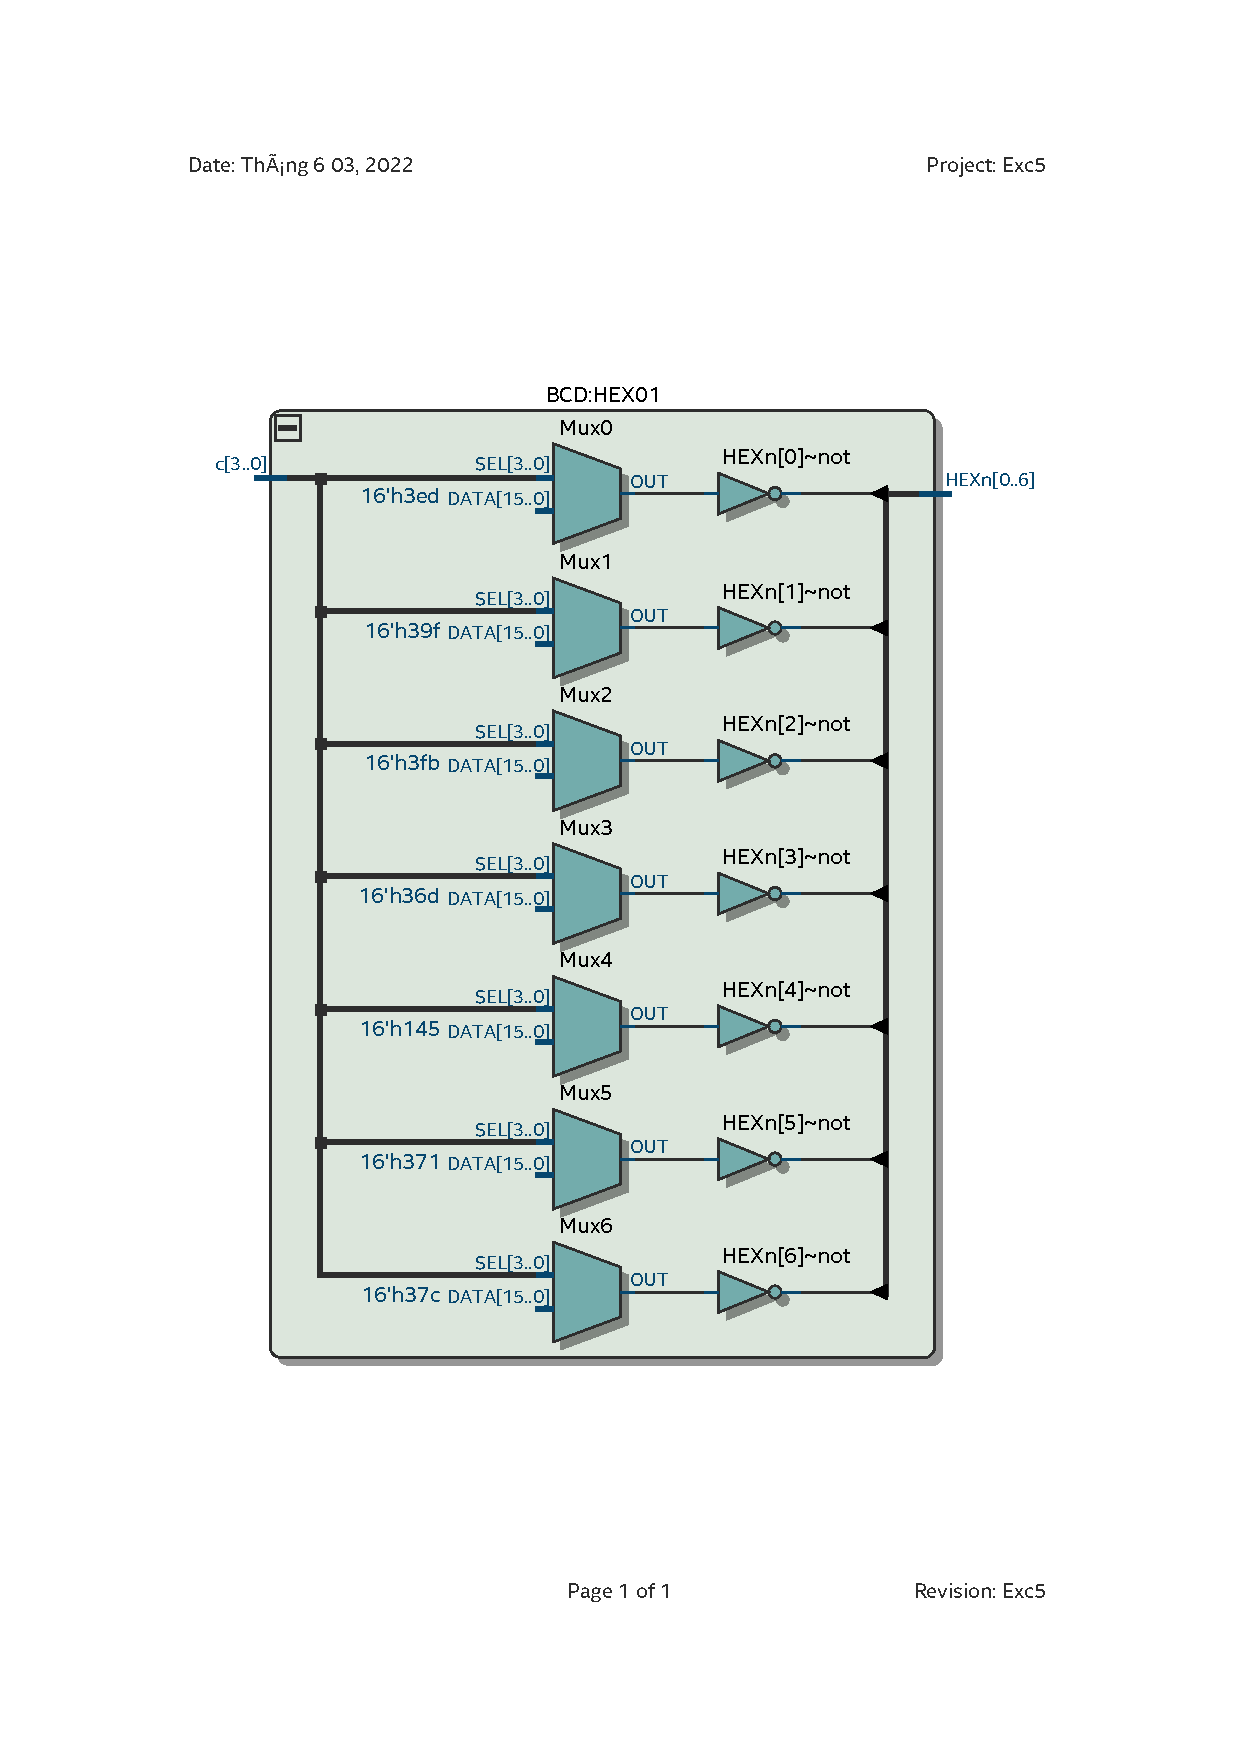
\includegraphics[scale=0.7, clip, trim={2cm 6.6cm 2cm 6.9cm}]{images/Exc5_BCD_RTL.pdf}
\caption*{BCD 7-segment decoder}
\end{figure}

\begin{figure}[H]
\centering
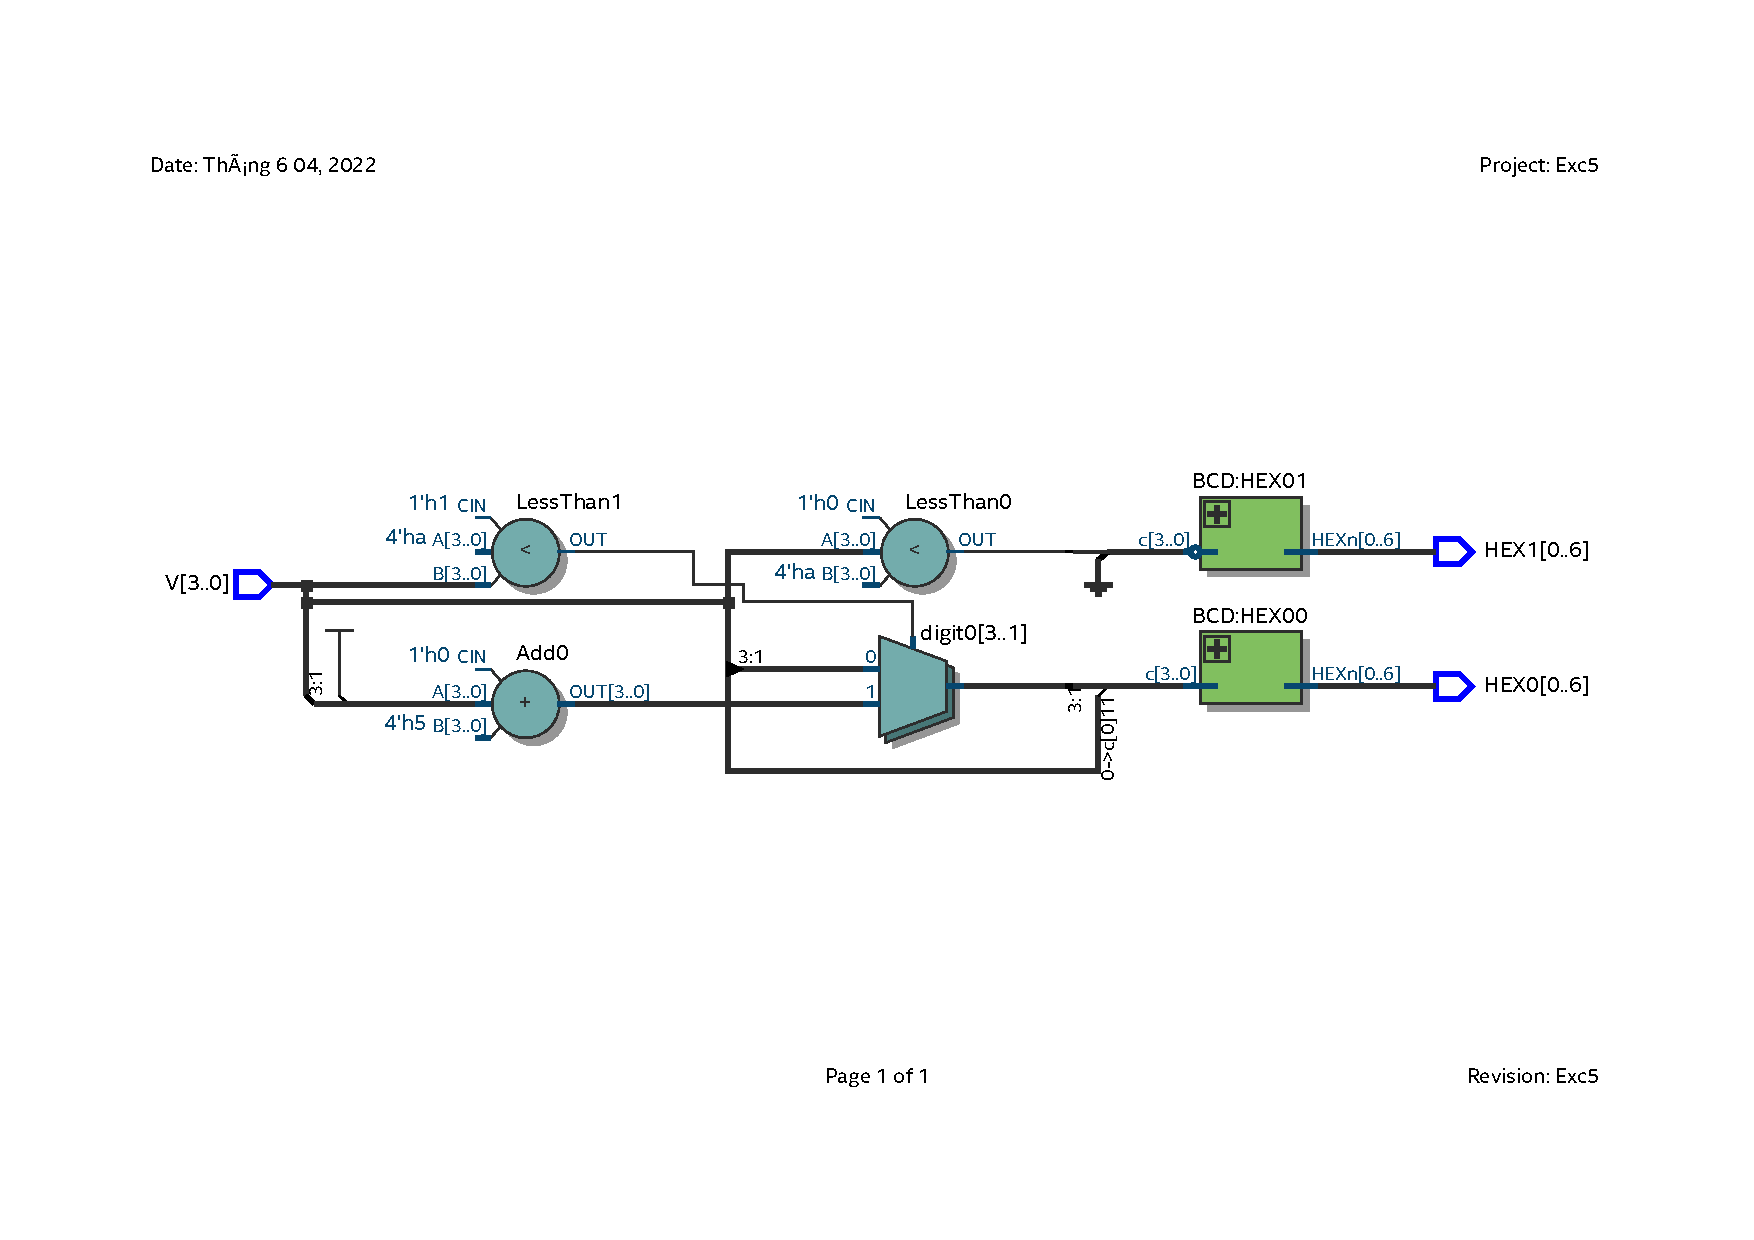
\includegraphics[scale=0.7, clip, trim={2cm 7cm 2cm 7cm}]{images/Exc5_RTL_2.pdf}
\caption*{Top level}
\end{figure}

\subsection{Waveform}
\begin{figure}[H]
\centering
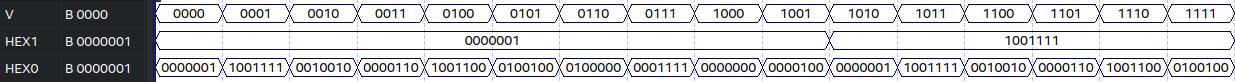
\includegraphics[scale=0.55]{images/Exc5_waveform.png}
\end{figure}

\end{document}